\chapter{Eulerian Domain: Finite Element Method}
\label{ch:eulerian}
	\lsymb[f]{$\mathcal{T}_h$}{Finite Element mesh}{-}{th}		
	\lsymb[f]{$T$}{Cell of Finite Element mesh}{-}{t}			
	
	\lsymb[f]{$v$}{Test function}{-}{v}				
	\lsymb[f]{$V$}{Trial vector function space}{-}{vte}				
	\lsymb[f]{$\hat{V}$}{Test vector function space}{-}{vtr}					
	\gsymb[f]{$\Omega$}{Fluid domain}{-}{x}	
	\gsymb[f]{$\Omega_E$}{Eulerian fluid domain}{-}{xe}	
	\gsymb[f]{$\Omega_L$}{Lagrangian fluid domain}{-}{xl}	
	\gsymb[f]{$\partial \Omega$}{Boundary of the domain $\Omega$}{-}{xdd}	

%------------------------------------------------------------------------------------------------------
%------------------------------------------------------------------------------------------------------
%------------------------------------------------------------------------------------------------------
%\section{Purpose of eulerian domain}
Standard \printAcron{Computation Fluid Dynamics}{CFD} method discretizes the fluid into smaller regions, known as grids, and solves the set of Navier-Stokes equations in this region. This type of formulation is referred to as an Eulerian method, as we are evaluating the change of flow property in a given volume.

For the hybrid method, we use the Navier-Stokes grid formulation in the near-body region. The advantage of using the Eulerian method at this region is that it is much more efficient in resolving the boundary layer than the Vortex Particle Method. We can directly enforce the wall boundary condition at the wall boundary of the Eulerian domain, solving the problem of vorticity generation of the body. In the hybrid coupling strategy, we can then interpolate this newly resolved near-wall solution on to the Lagrangian domain, where the vortex blobs can efficiently evolve the particles.

The various approaches to solve the fluid dynamics problem from a Eulerian reference frame. \indexAcron{Finite Volume Method }{FVM}, \indexAcron{Finite Difference Method}{FDM}, and \indexAcron{Finite Element Method}{FEM} are the common choice for solving the Navier-Stokes problem and differ by the way they approach to solve the problem. FVM divides the domain into volumes where it enforces the conservation of mass and momentum in each sub-domains. FDM divides the domain into nodes and use local Taylor expansions to approximate the partial differential equations. FEM divides the domain into elements and solves the problem using variational calculus. So in the end, the choice of Eulerian method does not have a direct impact on the coupling with the Lagrangian method as the purpose of the Eulerian method is only to efficiently, and accurately resolve the near-body region of the body.

We have decided to use the FEM packages provided by the \fenics project as they have be already implemented efficient, multi-threaded algorithms for solving the partial differential equation. Furthermore, they provide extensive features for future developments such as adaptive mesh refinement, fluid-structure interaction, and efficient computation of turbulent flow.

\section{Introduction to Finite Element Method}

\printAcron{Finite Element Method}{FEM} is numerical method to solve for the solution of a given partial differential equation. It is solved by describing it as a variation problem, giving us an approximate solution for the boundary value problem \cite{Brenner2002}. So the FEM approximates the unknown variables and converts the partial differential equations to a set of algebraic equations, which makes them easier to solve. It was traditionally used for solid mechanics (e.g for the analysis of aircraft structures \cite{RAO2011}), but have since then used to solve fluid dynamics problems \cite{Guermond2006a} \cite{Johnston2004a} \cite{Guermond2003a}.

\subsection*{Finite element discretization}

The finite element solves problem by dividing the domain of interest into smaller, simpler regions known as ``elements". These ``elements" are connected at the joints which are called nodes or nodal points. We use these sets of node and elements to represent the actual variation in the field (such as the displacement, the velocity, the pressure or the temperature) using simple functions, known as the basis functions. Thus, we have transformed the domain of interest into finite number of \indexAcron{Degrees of Freedom}{DOF}. We combine the set of equations of the element into a global system of equations to solve for the unknown.

	\begin{figure}[b]
	\centering
	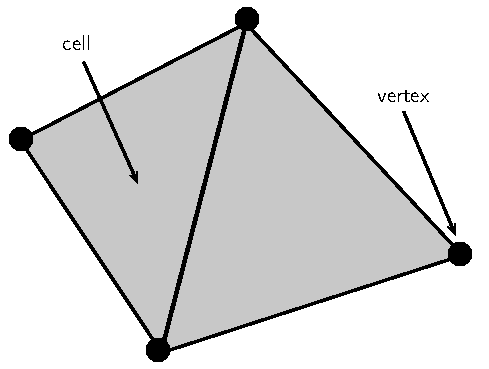
\includegraphics[width=0.4\linewidth]{./figures/eulerian/finiteElementDefinitions.pdf}
	\caption{A two-dimensional finite element geometry. The cell represents the area of the element, and vertices are the edges of the cell.}
	\label{fig:finiteElementDefinitions}
	\end{figure}

A finite element discretization in 2-D can be seen in figure \ref{fig:finiteElementDefinitions}. The figures shows two connected elements, where the cells represent the area of the element, and the vertices of the cell represents the nodes of the element. The finite number of cells $\mathcal{T}_h = \{T\}$ of the fluid domain $\Omega$, together makes the mesh of the Eulerian domain. As shown in figure \ref{fig:finiteElementDefinitions}, the cells of the finite element in 2-D, are made of simple geometrical shapes such as triangles or quadrilaterals. There are two approaches to discretize the domain: structured or unstructured mesh. The structured mesh has cells oriented in a structured pattern, and is the simplest approach in discretizing the mesh. The advantage of such a discretization is that it is possible to make a simple data structure which can be used to perform efficient computation. The downside to such discretization is that the mesh quality deteriorates as one increases the complexity of the domain. However, the FEM enables us to perform an unstructured discretization of the domain, as shown in figure \ref{fig:cylinderFiniteElementDiscretization}. The figure shows the unstructured discretization of the fluid domain around the cylinder $\Omega_E$, connecting the rectangular outer boundary of the fluid to the circular no-slip boundary of the body in a simple fashion. This shows that even though the unstructured method formulation is more complicated that the structured formulation, we have the advantage that the mesh quality does not deteriorate as the domain becomes more complex.

There are several algorithms for mesh generation. The standard approach is to employ the Delaunay triangulation method derived from the Voronoi diagram concept \cite{Carey1997}. This divides the domain into a set of triangles, as shown in figure \ref{fig:cylinderFiniteElementDiscretization}. This type of mesh generation allows us to connect different shapes of boundary with each other. Furthermore, this triangulation method be controlled by predefining the boundary element nodes using a transfinite interpolation.

\begin{figure}[t]
        \centering
        \begin{subfigure}[b]{0.5\textwidth}
                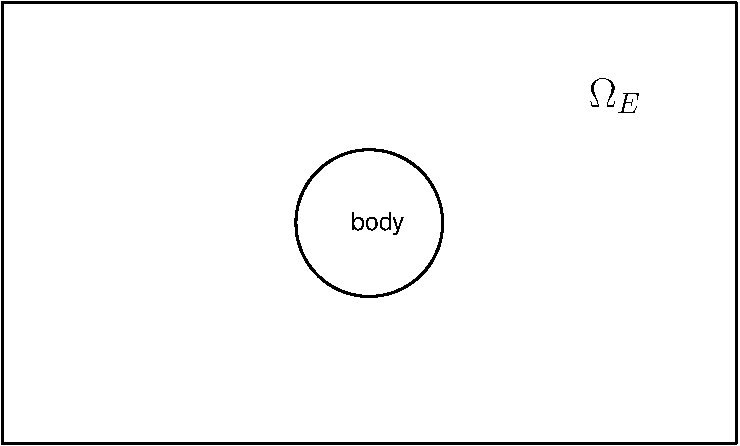
\includegraphics[width=\textwidth]{figures/eulerian/cylinderPreDelauney-crop.pdf}
                \caption{Fluid domain $\Omega_E$ around the cylinder}
                \label{fig:cylinderPreDelauney}
        \end{subfigure}%
        ~ %add desired spacing between images, e. g. ~, \quad, \qquad etc.
          %(or a blank line to force the subfigure onto a new line)
        \begin{subfigure}[b]{0.5\textwidth}
                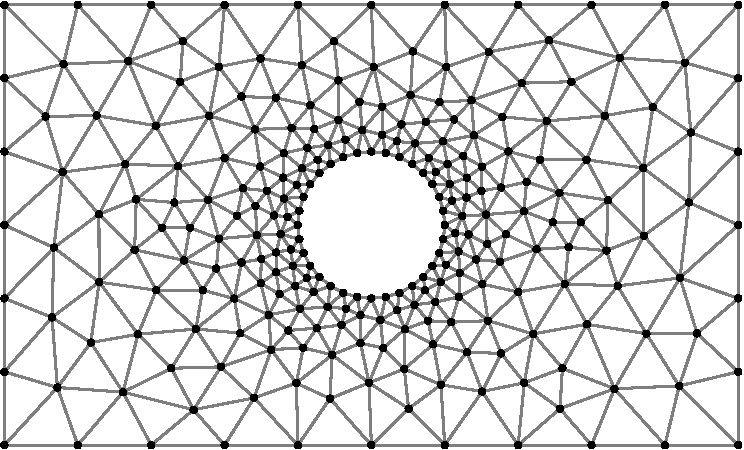
\includegraphics[width=\textwidth]{figures/eulerian/cylinderDelauney-crop.pdf}
                \caption{Delaunay triangulation of the fluid}
                \label{fig:cylinderDelauney}
        \end{subfigure}
        \caption{Delaunay triangulation of the fluid around a cylinder resulting in unstructured mesh with controllable cell sizes.}
        \label{fig:cylinderFiniteElementDiscretization}
\end{figure}	

\subsection*{Finite element function and function space}

The finite element is defined using a triple ($T, \mathcal{V}, \mathcal{L}$), as defined Ciarlet \cite{Ciarlet1972b} and used by the \fenics Project \cite{Logg2012b}. The domain $\Omega$ is divided into cells $T$, the space $\mathcal{V} = \mathcal{V}(T)$ is a finite dimensional function space on $T$ of dimension $n$, and $\mathcal{L} = \left\{ \ell_1,\ell_2,...,\ell_n \right\}$ is the set of degrees of freedom forming the basis for the dual space $\mathcal{V}'$ of $\mathcal{V}$.

When the domain $\Omega$ is divided into cells $T$, we can define the function and the function space of the finite element problem. For each cell, a local function space $\mathcal{V}$ can be defined to collectively construct the global function space $V$. Any given function $u \in V$ is a expressed in a linear combination of basis functions $\{\phi_1,\phi_2,...,\phi_N\}$,  of the function space $V$, 
	\begin{equation}
	u(x) = \sum_{j=1}^N U_j\phi_j(x).
	\end{equation}

There are several types of finite element families: the Brezzi-Douglas-Marini, the Crouzeiz-Raviart, the Discontinuous Lagrange, the Hermite, and the Lagrange elements \cite{Logg2012b}. Each has its own advantage such as the Discontinous Lagrange, or \indexAcron{Discontinous Galerkin}{DG} element consists of discontinuous functions, which was originally introduced for solving hyperbolic problem by Reed and Hill in 1973 \cite{Reed1973a}. The method was able to conserve mass at each element, had a high-order accuracy, and was robust in solving the advection problem. However for the current problem, we will rely on the Lagrange elements, also known as the \indexAcron{Continuous Galerkin}{CG}, which are based on the Lagrange polynomials \cite{Chen2011}. These elements are widely used and are the simplest to implement for our project. 

Lagrange elements belong to the space $H^1$, which a Sobolev space containing functions $u$ such that $u^2$ and $\left|\nabla u\right|^2$ have finite integral in the domain $\Omega$ \cite{Logg2012b}. The Lagrange element uses point evaluation for the degrees of the freedom, where a DOF in $(x,y)$ denotes the point evaluation of the function $u$, $\ell(u) = u(x,y)$. We can have a Lagrange elements of various orders $q = 1, 2,...$, where $q$ is the degree of the Lagrange polynomial $\mathcal{P}_q$ on the domain at $T$. For the 2-D case, the dimension $n$ of the finite element is given as,
	\begin{equation}
	n(q) = \frac{1}{2}(q + 1)(q + 2).
	\end{equation}

For $q=1$, we have a simple Lagrange element $\mathrm{CG}_1$, known as the Courant triange \cite{Courant1943}, with $3$ DOFs. For a higher order finite element, we can set $q=2$, giving us a Lagrange element $\mathrm{CG}_2$ with $6$ DOFs per cell. Figure \ref{fig:continuousGalerkin} shows the two Lagrange triangles $\mathrm{CG}_1$ and $\mathrm{CG}_2$ for $q = 1$ and $q=2$ respectively. The Courant triangle has the DOFs located at the vertices of the cell, and the higher order $\mathrm{CG}_2$ has $3$ additional DOFs, all located midway between the vertices. To describe our Eulerian problem of our hybrid scheme, we will rely on the $\mathrm{CG}_1$ and $\mathrm{CG}_2$ Lagrange elements.

	\begin{figure}[t]
	\centering
	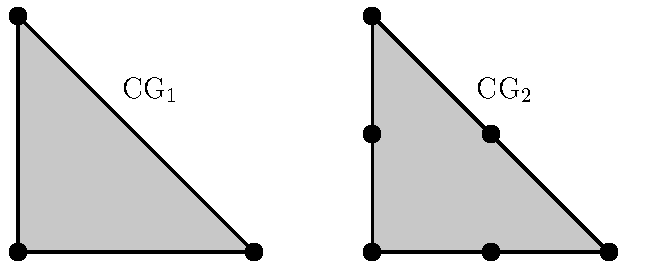
\includegraphics[width=0.6\linewidth]{./figures/eulerian/continuousGalerkin.pdf}
	\caption{The Lagrange $\mathrm{CG}_q$ triangle for $q = 1, 2$. The triangles have $3$ and $6$ DOFs respectively ({\color{black}{$\bullet$}}, black dot).}
	\label{fig:continuousGalerkin}
	\end{figure}



\subsection*{Variational formulation}
\label{subsec:variationalProblem}

To solve a basic problem such as a Poisson equation numerically, we need to convert it into a variational problem. The methodology is followed from the \fenics tutorial provide by Langtangen \cite{Logg2012b}. A 1D Poisson problem is given as,
	\begin{equation}
	\begin{aligned}
	- \nabla^2 u(x) &= f(x), \qquad x\ \mathrm{in}\ \Omega,\\
	u(x) &= u_0(x), \qquad x\ \mathrm{on}\ \partial\Omega.
	\end{aligned}
	\label{eq:poissonEq}
	\end{equation}
	
We can transform equation \ref{eq:poissonEq} into a variational form by multiplying it with a test function $v$, and integrating it over the domain $\Omega$,
	\begin{equation}
	- \int_{\Omega} \left(\nabla^2 u\right)v\ \mathrm{d}x= \int_{\Omega} fv\ \mathrm{d}x, \qquad \forall\ v \in \hat{V}.
	\label{eq:poissonEqVariationFormA}
	\end{equation}

In variational form equation \ref{eq:poissonEqVariationFormA}, the function $u$ is known as the trial function, and is what we are trying to approximate. The trial function $u$ lies in the trial function space $V$, and the test function $v$ lies in the test function space $\hat{V}$. When performing integration by parts, the test function $v$ is required to be zero at regions where $u$ is known. So, the additional terms cancel and we get,
	\begin{equation}
	- \int_{\Omega} \nabla u \nabla v\ \mathrm{d}x= \int_{\Omega} fv\ \mathrm{d}x \qquad \forall\ v \in \hat{V}
	\label{eq:poissonEqVariationFormB}
	\end{equation}

This form is referred to as the ``weak-form" of the original Poisson equation and is valid for all $v$ in the trial space $\hat{V}$. An inner product of any two function $f$ and $g$ in domain $\Omega$ is defined as,
	\begin{equation}
	\langle f,g \rangle = \int_{\Omega}fg\ \mathrm{d}x,
	\end{equation}
so we can simplify equation \ref{eq:poissonEqVariationFormB} to,
	\begin{equation}
	\langle \nabla u,\nabla v \rangle = \langle f,v \rangle, \qquad \forall\ v \in \hat{V}.
	\end{equation}

In order to solve this continuous problem numerically, we must transform it into a discrete variational problem,
	\begin{equation}
	-\langle \nabla u_h, \nabla v \rangle = \langle f, v \rangle \qquad \forall\ v \in \hat{V}_h \subset \hat{V},
	\label{eq:poissonEqDiscreteVariational}
	\end{equation}
where $u_h$ is the discrete function in the discrete space $V_h$ which is a subset of $V$, and the discrete function space $\hat{V}_h$ is a subset of $\hat{V}$. A common choice for the function space is the linear triangular element (Courant triangle) that has three nodes, as shown in figure \ref{fig:continuousGalerkin}, where $\hat{V}_h$ and $V_h$ are described by piecewise linear functions of the triangle. At the boundary, the functions in the test space is zero, whereas the functions in the trial space is equal the boundary condition $u_0$.  The equation \ref{eq:poissonEqDiscreteVariational} can be simplified as,
	\begin{equation}
	a\left(u,v\right) = L(v),
	\label{eq:weakForm}
	\end{equation}
where,
	\begin{equation}
	a\left(u,v\right) = - \langle \nabla u, \nabla v \rangle,
	\end{equation}
and
	\begin{equation}
	L(v) = \langle f,v \rangle.
	\end{equation}

The variable $a(u,v)$ and $L(v)$ is the denoted as the bilinear and linear form, respectively. For simplicity, we will ignore the discrete notation (i.e $\{\cdot\}_h \rightarrow \{\cdot\}$). To solve for the discrete solution we substitute,	
	\begin{equation}
	u = \sum_{j=1}^{N} U_j \phi_j,
	\label{eq:trialDiscrete}
	\end{equation}
the linear combination of the basis function $\phi_j$, spanning the function space $V$, into $a\left(u,v\right)$. The test function is a linear combination of the basis functions $\hat{\phi}_i$, spanning the test space $\hat{V}$, defined as,
	\begin{equation}
	v=\sum_{i=1}^{N} \hat{\phi}_i.
	\label{eq:testDiscrete}
	\end{equation}
	
The test function $v$ is taken to be zero at the boundary and one everywhere else. Substituting equation \ref{eq:trialDiscrete} and \ref{eq:testDiscrete} into equation \ref{eq:weakForm} gives,
	\begin{equation}
	\sum_{j=1}^N a(\phi,\hat{\phi}_i)\ U_j = L(\hat{\phi}_i).
	\end{equation}

Thus, we can solve the linear system of equations of form,
	\begin{equation}
	\mathbf{A}U = b,
	\label{eq:linearSysOfEq}
	\end{equation}	
where $\mathbf{A}_{ij} = a(\phi_j,\hat{\phi}_i)$ contains the coefficients, and the \printAcron{Right-Hand Side}{RHS} $b$ contains the knowns of the problem.
 	
\section{Solving the Finite Element problem}

To solve this linear system of equations, equation \ref{eq:linearSysOfEq}, we used \dolfin, the finite element library of the \fenics Project. This library uses high performance linear algebra kernels, and provide a scripting interface in \textsc{Python} for computational experience, ease similar to the \matlab interface. Such environment helps us to focus on the development of the theory (i.e the high-level algorithms). In order to generate the mesh of the fluid domain, we used \textsc{Gmsh}, a three-dimensional finite element mesh generator which proves a fast, light and user-friendly meshing tools.

\subsection{Introduction to FEniCS Project}

The \fenics Project is a collaborative work of various universities, that developed tools to perform automated finite element algorithms, which can be used to solve partial differential equation. It was a project originated in 2003 with the research collaboration of University of Chicago and Chalmers University of Technology with Logg,  Mardal, and Wells \cite{Logg2012b}. Since then, it has been expanded to various institutes such as Royal Institute of Technology, Simula Research Laboratory, University of Cambridge, and Delft University of Technology.

	\begin{figure}[p]
	\centering
	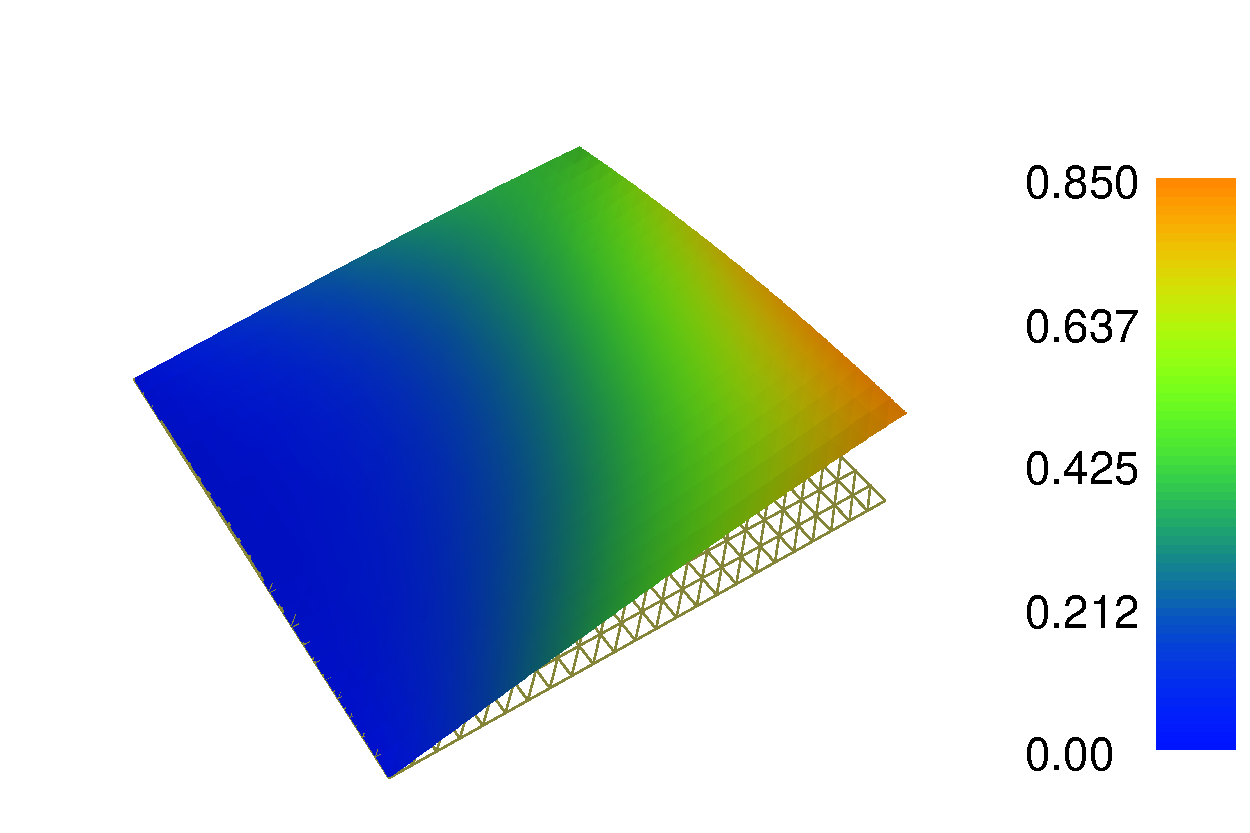
\includegraphics[width=0.5\linewidth]{./figures/eulerian/dolfinExampleFigure-rotated270.pdf}
	\caption{\dolfin VTK plot of the Poisson solution, given by the problem, source code listing \ref{lst:pycode-poisson}.}
	\label{fig:dolfinExampleFigure}
	\end{figure}

	\begin{listing}[p]
	\inputminted[fontseries=courier,obeytabs,fontsize=\footnotesize,mathescape,linenos,numbersep=5pt,frame=lines,framesep=2mm,xleftmargin=20mm,xrightmargin=20mm]{python}{figures/eulerian/dolfinExample.py}
	\caption{A complete program for solving the Poisson problem and plotting the solution. The Poisson problem is given as $-\nabla^2{u} = f$, where $u_0 = \sin{x}\cdot\cos{y}$ on the boundary and $f=2$. The code is written in \python using \dolfin 1.2 library}
	\label{lst:pycode-poisson}
	\end{listing}

The consists of various libraries such as UFC, UFL, FIAT, INSTANT and mainly \textsc{Dolfin}. \dolfin is the core library aimed at automating the solution of partial differential equations using finite element method \cite{Logg2010a}. It uses automated code generation thus maintaining high-level mathematical expressions but still providing efficient, multi-threaded performance (with \indexAcron{Message Passing Interface}{MPI}) internally. %It used built-in linear algebra backend such as PETSc, TRILINOS/EPECTRA, uBLAS, and MTL4.

We used the \dolfin library wrapped in \python to solve the finite element problem. For example, we can demonstrate the procedures of solving the Poisson problem, equation \ref{eq:poissonEq}. We can take $f=2$ with the boundary conditions,
	\begin{equation}
	u(x) = u_0(x) = \sin x \cdot \cos y,
	\end{equation}
at $\partial \Omega$. The finite element code generation is automated with \textsc{Dolfin}, leaving only the explicit expression of the problem in python, see source code listing \ref{lst:pycode-poisson}.

\subsection{Mesh generation using GMSH}
%The proper generation of the fluid mesh is an important aspect of the Finite Element method. It is an important process, as an ill-construct mesh can be computationally very expensive, or might even problem with convergence. There have been literatures dedicated just to improve the mesh generation, for example by Hansen \cite{Hansen2005}. It focused on mesh enhancement techniques for elliptical methods, which enables to increase the quality of the data, and also the robustness of the simulation.

The generation of the mesh is achieved by \textsc{Gmsh}, an open-source software developed by Geuzaine \& Remacle \cite{Geuzaine2009b}, which has implemented a user-friendly interface and fast algorithms. The \gmsh implemented kernels that use \textsc{BLAS} and LAPACK linear algebra packages in C++ for fast computation. Furthermore, it allows for scriptability making it ideal to integrate it with our current \python code project for future automation.

\section{Solving Incompressible Navier-Stokes Equations}
Using the \dolfin library for constructing the finite element problem, we can now solve the Eulerian method of our hybrid scheme. The Eulerian method will formulated the problem use the primitive variables velocity-pressure $\mathbf{u}-p$, which we can use to directly enforce the no-slip velocity boundary condition at the wall of the body. 

\subsection{Velocity-pressure formulation}
The velocity-pressure $\mathbf{u}-p$ formulation of the fluid, is the standard formulation of the Navier-Stokes equations of the fluid dynamics problem. The 2-D incompressible Navier-Stokes equations of a fluid with unit density (i.e $\rho = 1$) is given as,
	\begin{subequations}
	\begin{align}
	\frac{\partial \mathbf{u}}{\partial t} + \mathbf{u}\cdot\nabla\mathbf{u} - \nabla \cdot \sigma &= f,\\
	\nabla \cdot \mathbf{u} = 0,
	\end{align}	
	\label{eq:2Dns}
	\end{subequations}
where $\sigma$ is the Cauchy stress tensor defined as,
	\begin{equation}
	\sigma(\mathbf{u},p) = 2\nu\epsilon(\mathbf{u}) - p\mathbf{I}.
	\end{equation}

The Cauchy stress tensor is a function of pressure $p$, the fluid kinematic viscosity $\nu$, and the symmetric gradient $\epsilon$ defined as,
	\begin{equation}
	\epsilon(\mathbf{u}) = \frac{1}{2} \left(\nabla \mathbf{u} + \nabla \mathbf{u}^{\mathrm{T}}\right).
	\label{eq:symGrad}
	\end{equation}
describing the stresses in fluid due to the velocity gradient and the pressure. The incompressible 2-D Navier-Stokes equations have two unknowns, the vector velocity field $\mathbf{u}$, that lies on the vector-valued function space $V$, and the scalar pressure field $p$, which lies on the scalar-valued function space $Q$. Onces we solve these we can determine the vorticity field, which we will transfer to the Lagrangian domain. 

\subsection{Determining the vorticity field}

	\begin{listing}[t]
	\inputminted[fontseries=courier,obeytabs,fontsize=\footnotesize,mathescape,linenos,numbersep=5pt,frame=lines,framesep=2mm,xleftmargin=20mm,xrightmargin=20mm]{python}{figures/eulerian/vorticity.py}
	\caption{The \textsc{python} implementation of the vorticity calculation}
	\label{lst:pycode-vorticity}
	\end{listing}

The coupling between the Eulerian to Lagrangian method is through the transfer of the vorticity field $\omega$ from the Eulerian domain to the Lagrangian vortex blobs. The vorticity field $\omega$, is defined as,
	\begin{equation}
	\omega = \nabla \times u,
	\label{eq:vorticityEq}
	\end{equation}
and is defined as the curl of the velocity field $\mathbf{u}$, which lies on the scalar-valued function space $W$. Due to the constant change in the velocity field, we have to recalculate the vorticity at every time step $t_n, t_{n+1}, ...$ . To solve this problem in a efficient manner, we can use the \texttt{assemble} function of \dolfin to pre-construct the problem. We must first define the equation \ref{eq:vorticityEq} in the variational (integral) form,  
	\begin{equation}
	\int_{\Omega} \omega \cdot \mathbf{v}\ \mathrm{d}x = \int_{\Omega} (\nabla \times \mathbf{u},) \cdot \mathbf{v}\ \mathrm{d}x,
	\end{equation}
where $\omega = \sum_{j=1}^N \hat{\omega}_j\psi_j$, is a linear combination of basis function $\psi_j$, spanning the function space $W$. The variational form is summarized as,
	\begin{equation}
	a(\omega,\mathbf{v}) = L(\mathbf{u},\mathbf{v})
	\end{equation}
where $a(\omega,v)$ contains the knowns of the problem, which are fixed during the simulation. This can be pre-calculated to optimize the problem. $(\mathbf{u},\mathbf{v})$ is the unknown of the problem which has to be recalculated every time as it is a function of the current velocity. The \textsc{python} implementation of the algorithm is show in listing \ref{lst:pycode-vorticity}. Using the \dolfin library, we can used the \texttt{assemble} function to pre-calculated the LHS of the problem (line 10). So using the algorithms of the hybrid coupling scheme, we can transfer this vorticity field of the Eulerian domain on the vortex blobs.

\subsection{Taylor-Hood finite element family for solving ICNS}
To solve the \indexAcron{Incompressible Navier-Stokes}{ICNS} problem, we must choose an appropriate finite element function spaces for the velocity $\mathbf{u}$, the pressure $p$, and the vorticity $\omega$, by ensuring that we satisfy the Ladyzhenskaya-Babu\v{s}ka-Brezzi (LBB) compatibility condition, also known as the inf-sup compatibility condition \cite{Brezzi1991}. The Lagrange finite element spaces must have the order of velocity $q_{\mathrm{vel}}$, one order higher than the order of the pressure $q_{\mathrm{pres}}$,
	\begin{equation}
	q_{\mathrm{vel}} = 	q_{\mathrm{pres}} + 1.
	\end{equation}
Brezzi and Fortin \cite{Brezzi1991} showed that if both are of same order, it will result to an unstable problem. To solve the ICNS problem, we will used the Taylor-Hood family \cite{Taylor1973}, examined by Boffi \cite{Boffi1997}. The method use velocity order $q_{\mathrm{vel}} = 2$ and pressure order $q_{\mathrm{pres}} = 1$. We decided to choose this method, as it is the most conventional method, that is simple, and that shows a stable behavior.

In addition, we have to choose an appropriate function space for the vorticity. As vorticity is the curl of the velocity, to reduce interpolation error during the projection of the solution, we will used function space one order lower than the velocity, $q_{\mathrm{vort}} = 1$. Table \ref{tab:eulerianFunctionTerms} shows the list of the function spaces, the finite element type and their orders. In additional, we have included the variable names of the function space, trial functions and the test functions, associated to the function element that we have chosen for the problem.

	\ctable[
	    caption = {Summary of the Lagrange element $\mathrm{CG}_q$ of order $q$, that was used for solving the incompressible Navier-Stokes problem. The variable names of the function space, the trial functions, and the test functions are tabulated together.},
	    label   = {tab:eulerianFunctionTerms},
	    pos = t,
	]{lcccc}{}{\FL
	Variable	& Finite element & Function space	& Trial function & Test function \ML
	Velocity	& $\mathrm{CG}_2$	& $V$			& $\mathbf{u}$	 & $\mathbf{v}$\\
	Pressure 	& $\mathrm{CG}_1$ 	& $Q$			& $p$	 		 & $q$\\
	Vorticity 	& $\mathrm{CG}_1$	& $X$			& $w$	 		 & $x$\LL}


\subsection{Incremental pressure correction scheme}
\label{subsec:ipcs}
The algorithm to solve the NS problem was first demonstrated by Chorin in 1968 \cite{Chorin1968}, referred to as the Chorin's projection method or sometimes known as the non-incremental pressure correction scheme. The process relied on first computing a tentative velocity by initially neglecting the pressure in the momentum equation of the Navier-Stokes problem, equation \ref{eq:2Dns}. The velocity field is corrected by determining the pressure field satisfying a divergence free vector field. This method however does not satisfy the discrete incompressibility constraint exactly and so, Goda in 1979 \cite{Goda1979a}, introduced an improved \indexAcron{Incremental Pressure Correction Scheme}{IPCS}. The method computed the viscous term at the incremented time $(t_{n-1} + t_n)/2$, and used the stress formulation to determine the corrected pressure \cite{Logg2012b}. The detailed algorithms to the IPCS scheme, as demonstrated by the \fenics Project \cite{Logg2012b}, can be summarized as follows:

	\begin{enumerate}
	\item \textbf{Compute the tentative velocity:} The tentative velocity $\mathbf{u}^{\star}$ is determined by solving,
		\begin{equation}
		\begin{split}
		\langle D_t^n \mathbf{u}^{\star}, \mathbf{v} \rangle &+ \langle \mathbf{u}^{n-1}\cdot\nabla\mathbf{u}^{n-1},\mathbf{v}\rangle + \langle \sigma(\mathbf{u}^{n-\frac{1}{2}},p^{n-1}), \epsilon(\mathbf{v}) \rangle \quad \\ &\quad+ \langle p^{n-1}\hat{\mathbf{n}},\mathbf{v}\rangle_{\partial \Omega} - \langle \mathbf{v}\ \hat{\mathbf{n}} \cdot (\nabla \mathbf{u}^{n-\frac{1}{2}} )^{\mathrm{T}},\mathbf{v} \rangle_{\partial \Omega} = \langle f^n,\mathbf{v} \rangle,
		\end{split}
		\label{eq:tentativeVel}
		\end{equation}
	is valid for all $\mathbf{v} \in V$, where $\mathbf{u}^{n-\frac{1}{2}}$ is defined as,
		\begin{equation}
		\mathbf{u}^{n-\frac{1}{2}} = \frac{\mathbf{u}^{\star}+\mathbf{u}^{n-1}}{2},
		\end{equation}
	With the Dirichlet velocity boundary conditions at the boundary $\partial \Omega$, we can solve the equation \ref{eq:tentativeVel}. The additional term,
		\begin{equation}
		\langle \mathbf{v}\ \hat{\mathbf{n}} \cdot (\nabla \mathbf{u}^{n-\frac{1}{2}} )^{\mathrm{T}},\mathbf{v} \rangle_{\partial \Omega},
		\end{equation}
	is resulted from the integration by parts, when we evaluate the viscous term at $(t_{n-1} + t_n)/2$ and we use the stress formulation instead of the Laplacian formulation as done for the Chorin scheme. This difference ensures that the velocity profile at the inlet and the outlet of the domain is more accurate that the ones obtained for the Chorin scheme. 
	
	The source code for solving the tentative velocity problem is shown in listing \ref{lst:pycode-tentativeVelocity}. First, we pre-define all the terms need for the tentative velocity problem formulation (lines \numrange{3}{16}). We can also pre-assemble the LHS of the problem (line 19) outside of the time-integration loop, as it remains constant. During the time integration, we first assemble the RHS of the problem (line 26), then apply the Dirichlet velocity boundary condition (line 29) which consist of the wall boundary condition, and external Dirichlet velocity boundary condition (e.g. the free-stream). Finally, we can solve the problem using GMRES solver for solving the system of linear equations.
	
		\begin{listing}[t]
		\inputminted[fontseries=courier,obeytabs,fontsize=\scriptsize,mathescape,linenos,numbersep=5pt,frame=lines,framesep=2mm,xleftmargin=20mm,xrightmargin=20mm]{python}{figures/eulerian/tentativeVelocity.py}
		\caption{The source code for solving the tentative velocity $\mathbf{u}^{\star}$, using the equation \ref{eq:tentativeVel}}
		\label{lst:pycode-tentativeVelocity}
		\end{listing}
	
	\item \textbf{Determine the corrected pressure:} The corrected pressure $p^n$ is determined by solving,	
		\begin{equation}
		\langle \nabla p^n, \nabla q \rangle = \langle \nabla p^{n-1}, \nabla q\rangle - \langle \nabla \cdot \mathbf{u}^{\star}, q \rangle / \Delta t_n
		\label{eq:pressureCorrection}
		\end{equation}
	valid for all $q \in Q$. We use the previously calculated tentative velocity $\mathbf{u}^{\star}$ to determine the corrected pressure. We can solve the problem using the Neumann pressure boundary condition at the pressure outlet of the domain. We define a boundary as the pressure outlet, if we do not know the velocity boundary condition at that boundary. This is true for the region were the exit flow is perturbed. However, for the coupled Eulerian method (that we will use), all the boundary conditions are available as a velocity boundary condition from the Lagrangian domain. This means that do not have to assume any pressure boundary condition.

	The source code for solving the corrected pressure problem is shown in listing \ref{lst:pycode-correctedPressure}. As done for the tentative velocity, we can formulate and pre-assemble the problems before the time loop. In the time loop, we only need to assemble the RHS, apply the boundary condition (if it exists), and finally solve for the corrected pressure. Using the corrected pressure, we can determine the corrected velocity field. 
		
		\begin{listing}[p]
		\inputminted[fontseries=courier,obeytabs,fontsize=\scriptsize,mathescape,linenos,numbersep=5pt,frame=lines,framesep=2mm,xleftmargin=20mm,xrightmargin=20mm]{python}{figures/eulerian/correctedPressure.py}
		\caption{The source code for solving the corrected pressure $p^n$ using the equation \ref{eq:pressureCorrection}}
		\label{lst:pycode-correctedPressure}
		\end{listing}
			
	\item \textbf{Determine the corrected velocity:} The corrected velocity field $u^n$ is determined by solving,
		\begin{equation}
		\langle \mathbf{u}^n, \mathbf{v}\rangle = \langle \mathbf{u}^{\star},\mathbf{v} \rangle - \Delta t_n \langle \nabla(p^n - p^{n-1}),\mathbf{v} \rangle,
		\end{equation}
	which is valid for all $\mathbf{v} \in V$. We correct the tentative velocity $\mathbf{u}^{\star}$ by the pressure difference to determine the correct velocity field. We will have to apply the Dirichlet velocity boundary condition at the boundary again, to solve for the problem.
	
	The source code of the solving the corrected pressure problem in shown in listing \ref{lst:pycode-correctedVelocity}. We first initialize the problem, by formulating the problem and assembling the LHS outside the time loop (line \numrange{3}{8}). In the time integration loop, we assemble the RHS, apply the velocity boundary condition and finally solve for the corrected velocity field.
	
		\begin{listing}[p]
		\inputminted[fontseries=courier,obeytabs,fontsize=\scriptsize,mathescape,linenos,numbersep=5pt,frame=lines,framesep=2mm,xleftmargin=20mm,xrightmargin=20mm]{python}{figures/eulerian/correctedVelocity.py}
		\caption{The source code for solving the corrected pressure $p^n$ using the equation \ref{eq:pressureCorrection}}
		\label{lst:pycode-correctedVelocity}
		\end{listing}
		
	\end{enumerate}
	
This algorithm was implemented using \textsc{Dolfin}'s Krylov \textsc{Gmres} solver with an absolute and a relative error tolerance of \num{e-25} and \num{e-12} respectively. The program structure was based on the collection of benchmark and solvers provided by the \fenics examples scripts \cite{nsbench}. The algorithm described above an explicit time marching scheme, \indexAcron{Forward Euler}{FE}, the simplest time marching scheme. Therefore, for the time marching scheme to be stable, we require the CFL number to satisfy the following condition:
	\begin{equation}
	\mathrm{CFL} = \Delta t_{\mathrm{max}} \frac{\lVert\mathbf{u}\rVert_{\mathrm{max}}(\nu +  \Delta h_{\mathrm{min}}\lVert\mathbf{u}\rVert_{\mathrm{max}})}{\Delta h_{\mathrm{min}}^2} \leqslant 1.
	\label{eq:cfl}
	\end{equation}
	
This gives us the direct constraint on the maximum Eulerian time step size $\Delta t_{E,\mathrm{max}}$ which is function of the $\mathrm{CFL}$ number, maximum fluid velocity in the Eulerian domain $\lVert \mathbf{u} \rVert_{\mathrm{max}}$, the fluid viscosity $\nu$ and the minimum mesh cell size $\Delta h_{min}$. 

%When coupling with the Lagrangian method, we will see that $\Delta t_E \leqslant \Delta t_L$ (Lagrangian time step size is ideally larger than Eulerian time step size), meaning that we will have to perform $k_E$ Eulerian sub-steps to reach the Lagrangian step, figure \ref{fig:multiStep}.

\subsection{Determining the body forces}

	\begin{listing}[t]
	\inputminted[fontseries=courier,obeytabs,fontsize=\footnotesize,mathescape,linenos,numbersep=5pt,frame=lines,framesep=2mm,xleftmargin=20mm,xrightmargin=20mm]{python}{figures/eulerian/forces.py}
	\caption{The \textsc{python} implementation of the force calculation}
	\label{lst:pycode-forceCalculation}
	\end{listing}

After we determine the flow fields, we can perform comparisons on the lift and the drag generated by the body. To determine there parameters, we first need to determine the friction and pressure forces acting on the no-slip boundary, which can be determined from the stress tensor $\sigma$ acting on the surface of the body. The stress tensor $\sigma$ is given by,
	\begin{equation}
	\sigma(\mathbf{u},p) = 2\nu\epsilon(\mathbf{u}) - p\mathbf{I},
	\end{equation}
where $\epsilon$ is the symmetric gradient, equation \ref{eq:symGrad}, and is a function of the velocity $\mathbf{u}$ and the pressure $p$ acting on the surface.The lift coefficient and the drag coefficient is computed as,
	\begin{subequations}
	\begin{align}
	L &= \int_{\partial \Omega} \left[\sigma(\mathbf{u},p) \cdot \hat{\mathbf{n}}\right]\cdot \hat{\mathbf{e}}_y\ \mathrm{d}s,\\
	D &= \int_{\partial \Omega} \left[\sigma(\mathbf{u},p) \cdot \hat{\mathbf{n}}\right]\cdot \hat{\mathbf{e}}_x\ \mathrm{d}s,
	\end{align}
	\label{eq:LiftDragEq}
	\end{subequations}
where $\hat{\mathbf{e}}_x$ and $\hat{\mathbf{e}}_y$ are the 2D unit Cartesian vectors,
	\begin{equation}
	\hat{\mathbf{e}}_x = \begin{bmatrix}
	 1 \\ 
	 0 
	\end{bmatrix}, \qquad \quad 
	\hat{\mathbf{e}}_y = \begin{bmatrix}
		 0 \\ 
		 1 
		\end{bmatrix}.\\
	\end{equation}

The lift coefficient and the drag coefficient, $C_l$ and $C_d$ respectively, is the lift and drag normalized with the dynamics pressure and reference length $c$ (in 2D), where the lift perpendicular to the free-steam and the drag is tangential to it,
		\begin{equation}
		C_l = \frac{L}{\frac{1}{2}\lVert\mathbf{u}\rVert_{\infty}^2 c},\qquad \quad
		C_d = \frac{D}{\frac{1}{2}\lVert\mathbf{u}\rVert_{\infty}^2 c}.\\
		\label{eq:LiftDragCoeffEq}
		\end{equation}

\section{Validation of eulerian method}
To validate our Eulerian method, we will first investigate the problem of the Lamb-Oseen vortex. Then we will compare the results of the Clercx-Bruneau dipole collision at $Re=625$. Finally, we will investigate the problem of the Impulsively started cylinder at $Re=550$, which we can use to validate the evolution of lift and drag.

\subsection{Lamb-Oseen Vortex}

	\ctable[
		caption = {Summary of the parameters for the Lamb-Oseen vortex evolution.},
		label   = {tab:eulerianLambOseenParams},
		pos = t,]{lcll}{}{\FL
		
		Parameters 					& Value 	& Unit					& Description \ML
		$\Gamma_c$\T               	& 1 &\si{m^2.s^{-1}} 				& Core strength\\
		$\Omega$               		& $\left[-1,1\right]^2$ &\si{m}		& Eulerian domain bounds \\
		$\mathbf{u}_{\infty}$ 		& $\left[0, 0\right]$ &\si{m.s^{-1}} & Free-stream velocity\\
		$\nu$						& $\num{5e-4}$ &\si{kg.s^{-1}.m^{-1}}& Kinematic viscosity\\
		$ (\tau_0,\tau_f)$ 		    & \numrange{2e-3}{2.5e-3} &\si{m^2}	& Initial and final scaled viscous time\\
		$ (t_0,t_f)$ 		    	& \numrange{4}{5} &\si{s}			& Initial and final simulation time\\		
		$ h_{\mathrm{min}}$			& $\frac{1}{100}\sqrt{2}$ &\si{m}			& Minimum mesh cell size\\	        
		$ N_{\mathrm{cells}}$ 		& $200^2$ 	& -						& Number of mesh cells\\
		$ \mathrm{CFL}$								& $0.95$ & -		& CFL number\\	        	        
		$\lVert \mathbf{u} \rVert_{\mathrm{max}}$	& $1.5$	& 	\si{m.s^{-1}} & Maximum magnitude fo the velocity\\		
		$ \Delta t$ 				& $0.001$ &\si{s}					& Time step size\\
		$ N_{\mathrm{t-steps}}$ 	& 1000 & -							& Number of time integration steps\\
		$\mathrm{ID}_{\mathrm{fluid}}$ & $1$ & - & Fluid domain I.D\\
		$\mathrm{ID}_{\mathrm{ext}}$ & $3$ & - & External Dirichlet velocity boundary I.D\LL}

The Lamb-Oseen vortex is an analytical solution by Lamb and Oseen, describing the diffusion of a vortex core \cite{Tryggeson2007}. We solved the same problem as the one described in the Lagrangian validation problem \ref{subsec:lagrangianLambOseen}. 

\subsubsection*{Problem Definition}
In the Lagrangian method, the Lamb-Oseen vortex was initialized using the vorticity field as the vortex blobs carry circulation strengths. However, Eulerian domain use the primitive variables $\mathbf{u}-p$ for formulating the problem. Therefore, we use the Lamb-Oseen velocity field as the initial conditions for the problem. The velocity field is given as,
	\begin{subequations}
	\begin{align}
	u_{\theta} &= \frac{\Gamma_c}{2\pi r} \left[1-\exp\left(-\frac{r^2}{4\tau}\right)\right]\\
	u_r &= 0,
	\end{align}
	\end{subequations}
where $\Gamma_c$ is the vortex core strength, $\tau \equiv \nu t$ is the scaled viscous time, and $r$ is the distance from the core center. The parameters of the simulation is tabulated in table \ref{tab:eulerianLambOseenParams}. To ease the comparison of the Eulerian to the Lagrangian method, we performed ensure similar spatial resolution. The figure \ref{fig:lambOseenDomainDefinition} shows the domain of the problem, discretized the domain $\Omega = \left[-1,1\right]^2$ in a structure grid with the number of finite element cells $N_{\mathrm{cells}}=200^2$ in $x$ and $y$ direction, minimum cell size $h=\sqrt{2}/100$. 

	\begin{figure}[t]
	\centering
	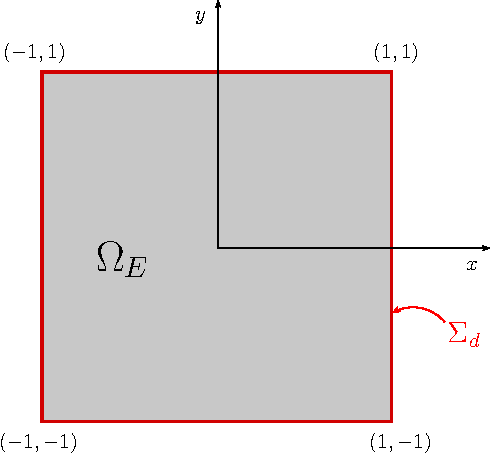
\includegraphics[width=0.5\linewidth]{./figures/eulerian/lambOseenDomainDefinition-crop.pdf}
	\caption{Eulerian domain for the Lamb-Oseen vortex problem. Figure shows the bound of the domain $\Omega = \left[-1,1\right]^2$, identified as $\mathrm{ID}_{\mathrm{fluid}} = 1$; and the boundary domain $\partial \Omega$ [{\color{plotRed}{---}}, solid red], identified as  $\mathrm{ID}_{\mathrm{ext}} = 3$, which is where the Dirichlet velocity boundary condition was applied.}
	\label{fig:lambOseenDomainDefinition}
	\end{figure}

Furthermore, the figure \ref{fig:lambOseenDomainDefinition} also shows the boundary domains $\partial \Omega$ of the fluid domain. For the Lamb-Oseen problem, as we have the analytical solution of the velocity field for all time, we can use this solution to prescribe the external domain boundary condition. So for this problem, we only need an external Dirichlet velocity boundary condition, at the boundary domain identified as, $\mathrm{ID}_{\mathrm{ext}} = 3$. This would imply that we do not need to explicitly apply the pressure boundary condition, as we already have a velocity boundary condition. With all the boundary conditions, we can evolve the initial velocity distribution of the Lamb-Oseen vortex from $t_0 = 4$ to $t_f =5$, using the IPCS algorithm described in section \ref{subsec:ipcs}. 

	\begin{figure}[p]
	\centering
	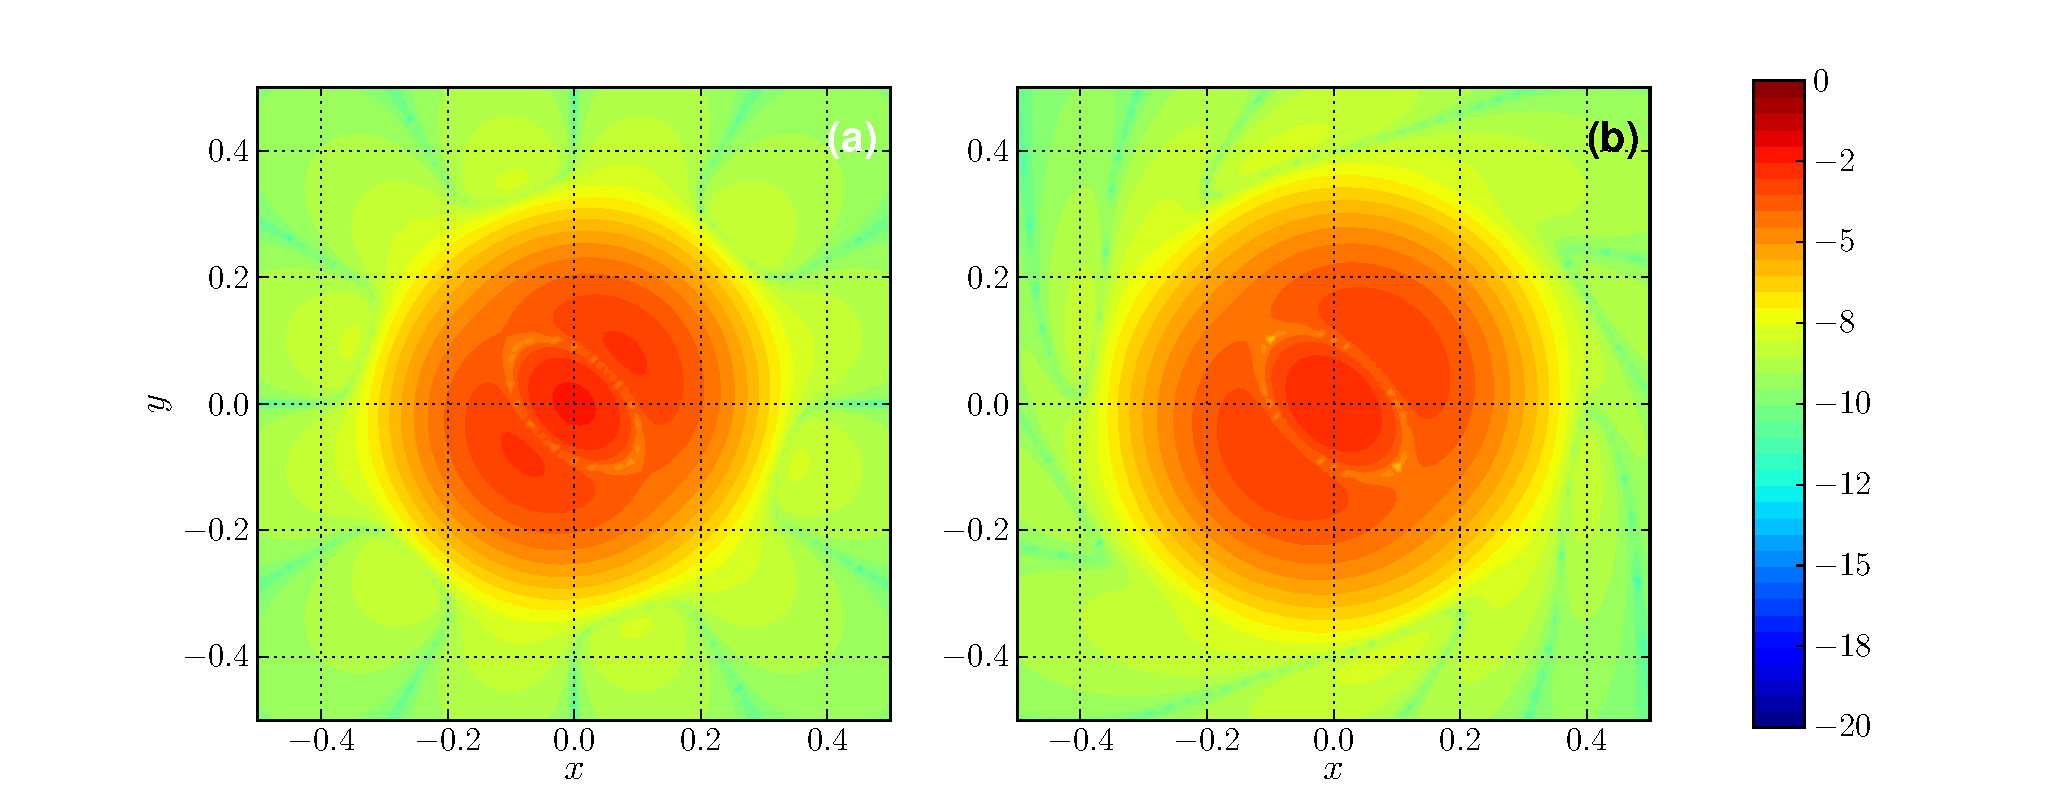
\includegraphics[width=0.99\linewidth]{./figures/eulerian/lambOseen_eulerian_wRelField_compressed.pdf}
	\caption{Relative error in vorticity field in logarithmic scale. Figure \textbf{(a)} shows the initial relative error in vorticity at $t=t_0$, and figure \textbf{(b)} shows the relative error in vorticity at the end of the time stepping $t=t_f$.}
	\label{fig:lambOseen_eulerian_wRelField_compressed}
	\end{figure}
	
	\begin{figure}[p]
	\centering
	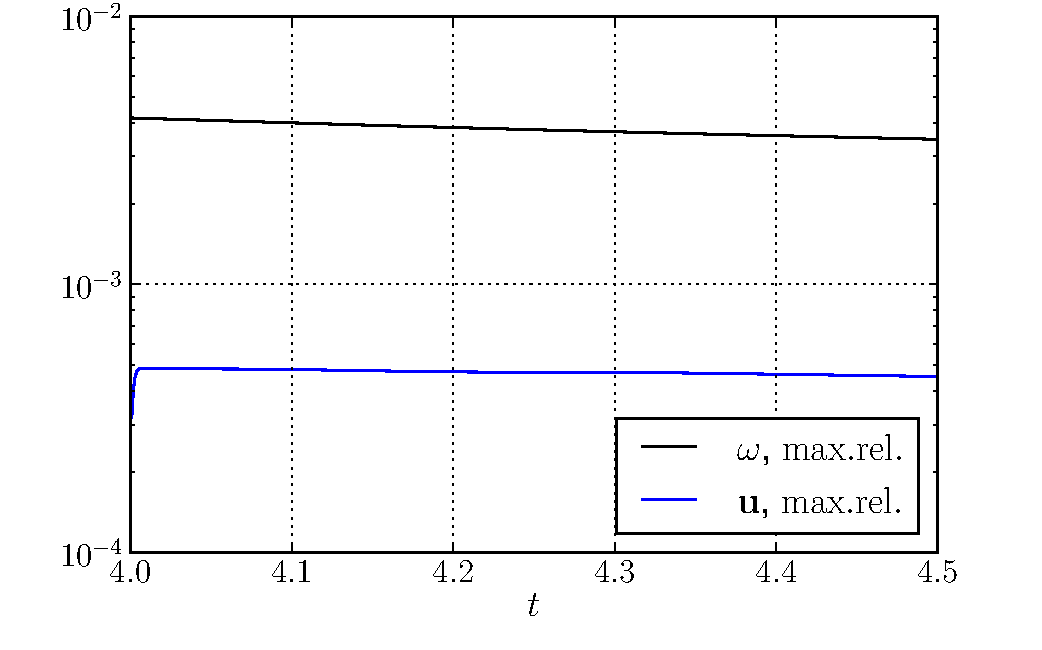
\includegraphics[width=0.6\linewidth]{./figures/eulerian/lambOseen_eulerian_wRelEvolution_compressed.pdf}
	\caption{Evolution of the maximum relative errors from $t_0=4$ to $t_f=4.5$. The figure depicts maximum relative error in velocity [{\color{plotBlue}{---}}, solid blue] and the maximum relative error in vorticity [---, solid black].}
	\label{fig:lambOseen_eulerian_wRelEvolution}
	\end{figure}

	\begin{figure}[p]
        \centering
        \begin{subfigure}[b]{0.5\textwidth}
                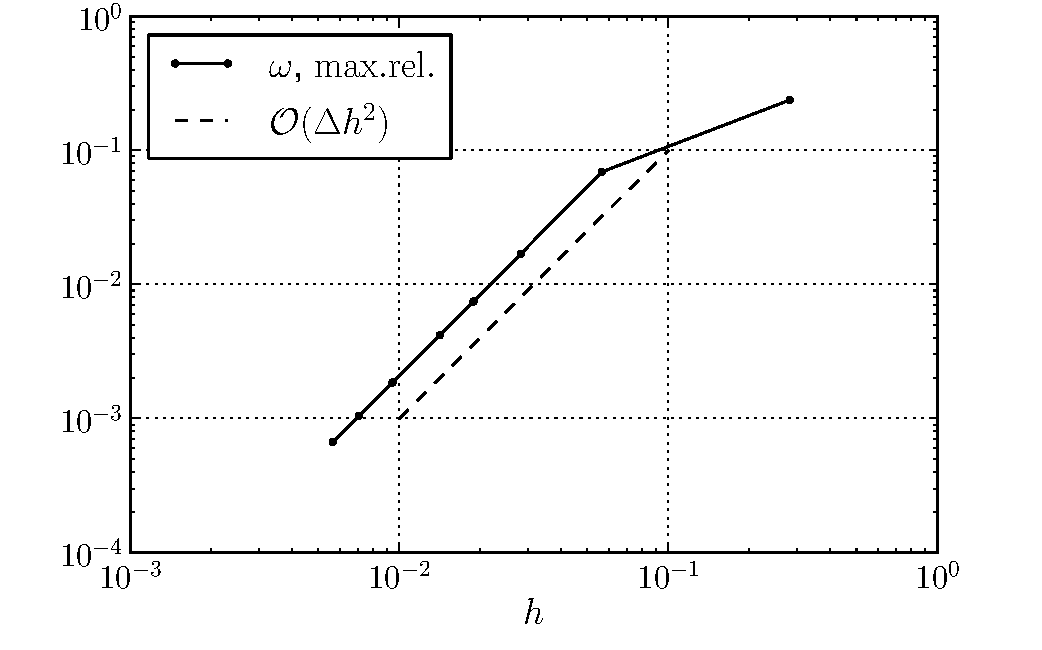
\includegraphics[width=\textwidth]{figures/eulerian/lambOseen_eulerianConvergence_dx_compressed.pdf}
                \caption{Spatial convergence}
                \label{fig:lambOseen_eulerianConvergence_dx}
        \end{subfigure}%
        ~ %add desired spacing between images, e. g. ~, \quad, \qquad etc.
          %(or a blank line to force the subfigure onto a new line)
        \begin{subfigure}[b]{0.5\textwidth}
                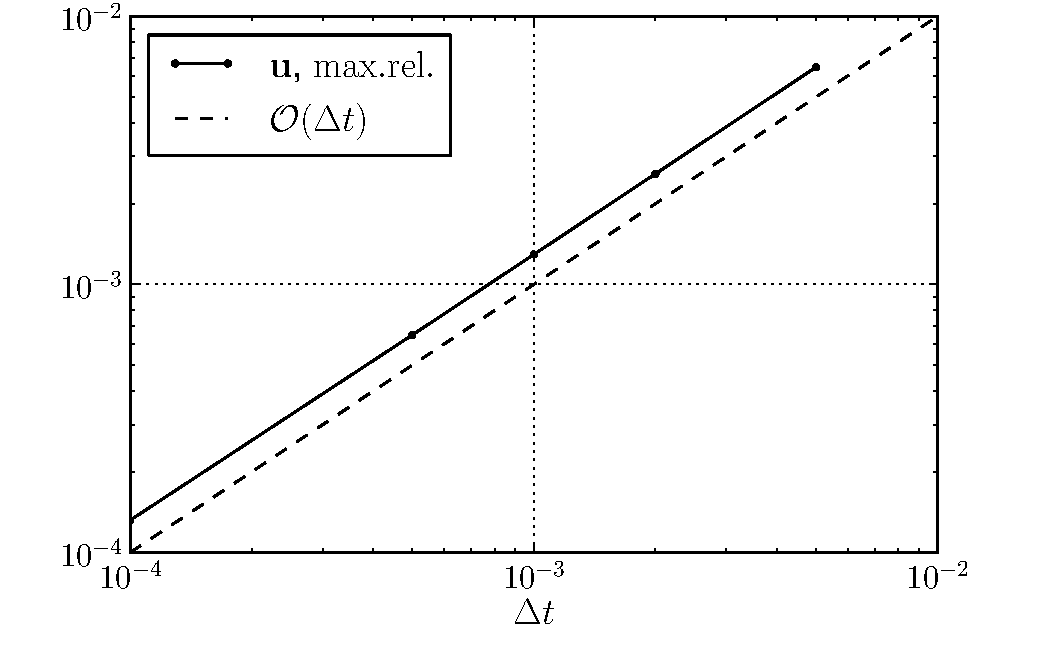
\includegraphics[width=\textwidth]{figures/eulerian/lambOseen_eulerianConvergence_dt_compressed.pdf}
                \caption{Temporal convergence}
                \label{fig:lambOseen_eulerianConvergence_dt}
        \end{subfigure}
        \caption{Convergence in space and time. The figure depicts \textbf{(a)} convergence in space of $\mathcal{O}(\Delta h^2)$ and \textbf{(b)} convergence in time of $\mathcal{O}(\Delta t)$.}
        \label{fig:lambOseen_eulerianConvergence}
	\end{figure}		
	

We used $CFL$ stability condition equation \ref{eq:cfl}, to determine the time step size, $\Delta t = 0.001$. The Eulerian method time steps using a \printAcron{Forward Euler}{FE} time marching and requires $N_{\mathrm{t-steps}}=1000$ time steps. During the evolution, we evaluated the growth of the error in velocity, and in vorticity between the numerical results and the analytical solution. 

\subsubsection*{Results}
We are interested in the evolution of error in vorticity, as this is the quantity which will be interpolated onto the Lagrangian domain. Figure \ref{fig:lambOseen_eulerian_wRelField_compressed} shows the initial and the final relative error in vorticity over the Eulerian domain. Opposed to the Lagrangian results, figure \ref{fig:lambOseen_convection_vorticityErrorContours_compressed}, we see that initial relative error in the vorticity field is larger. This is so because, the Lagrangian domain was initialized using the vorticity, where as the Eulerian domain was initialized using the velocity. To calculate the vorticity on the Eulerian domain, we had to project the curl the velocity onto the function space of vorticity $W$. This process of initialization in the finite element domain and project of the vorticity introduced additional numerical error. However, the pattern of the relative error in vorticity, is similar to the Lagrangian solution, with highest error at the core center, where we have the highest gradients in vorticity.

As the time progress, we see that the error of the problem is stable and does not increase as observed for the Lagrangian domain, figure \ref{fig:lambOseen_eulerian_wRelField_compressed}b. The growth of the relative error in velocity and vorticity can be observed in figure \ref{fig:lambOseen_eulerian_wRelEvolution}. It shows that during the evolution of the Lamb-Oseen vortex, the relative error in velocity, and vorticity is stable. We see that due to the relation of vorticity to velocity, the error in vorticity is higher that velocity.

To determine the convergence of space, the simulation was run for $h \approx 0.25$ to $h \approx \num{5e-3}$. Figure \ref{fig:lambOseen_eulerianConvergence_dx} shows the convergence of the relative error in vorticity. This validates that the scheme is $2^{nd}$-order in space, due to second order function space $CG_2$ for the primitive variable, velocity.

To determine convergence in time, we ran the simulation with various time steps $\Delta t = \num{5e-3}$ to $\Delta t = \num{1e-4}$). As we performed the investigation, we saw that the error in primitive variable $\mathbf{u}$, converged at an order 1, figure \ref{fig:lambOseen_eulerianConvergence}. This is true to the theory, as we are employing a $1^{\mathrm{st}}$-order Forward Euler scheme for the time integration. Thus, we have verified with the analytical solution of the Lamb-Oseen vortex that our Eulerian method is implemented according to the theory, and perform in a robust manner.

\subsection{Clercx-Bruneau dipole collison at $Re=625$}

The Eulerian method that we have developed here is to be used a wall-bounded Eulerian solver that can highly resolve the vorticity production of the boundary for the Hybrid method. Therefore it is vital that the vortex interaction with the no-slip boundary is handled properly.

To determine the proper handling of the no-slip boundary, it is common practice to use a simple test of dipole colliding with the wall. In this test cases, one could observe how the no-slip boundary handles the incoming vortex and can be used to determine if the system is formulated appropriately.  Ould-salihi et al. \cite{Ould-Salihi2001a} used this case to validate their Hybrid method that couples vortex particles with finite-difference method. Cottet et al. \cite{Cottet2000b} used the collision to tool to validate the vortex method. Therefore, we decided to use the Clercx-Bruneau dipole collision is a test case from Clercx \& Bruneau \cite{Clercx2006a}, where they performed a numerical study of a normal collision of a dipole with a no-slip boundary. This experiment provide extensive benchmark results for various Reynolds numbers with a Chevyshev pseudo-spectral numerical method. 

\subsubsection*{Problem Definition}

Unlike other dipole test cases, Clercx \& Bruneau provide well-defined initial and boundary conditions for the dipole vorticity field. Furthermore, they used a vorticity distribution that was continuous, which ensures a smooth velocity field for our Eulerian method using the $\mathbf{u}-p$ formulation. The literature provided results for the collision that we are interested: a normal collision with the dipole traveling perpendicular to the wall.

	\begin{figure}[t]
     \centering
     \begin{subfigure}[t]{0.45\textwidth}
             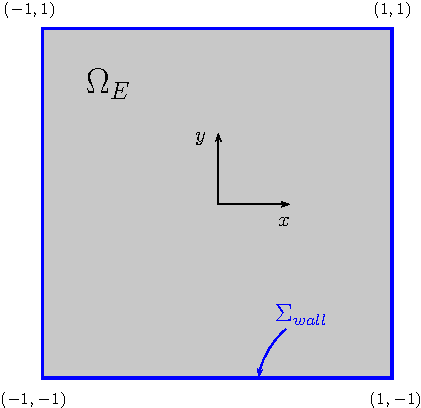
\includegraphics[width=\textwidth]{figures/eulerian/clercxBruneauDomainDefinition-crop.pdf}
             \caption{Domain definition}
             \label{fig:clercxBruneauDomainDefinition}
     \end{subfigure}%
     ~ %add desired spacing between images, e. g. ~, \quad, \qquad etc.
       %(or a blank line to force the subfigure onto a new line)
     \begin{subfigure}[t]{0.45\textwidth}
             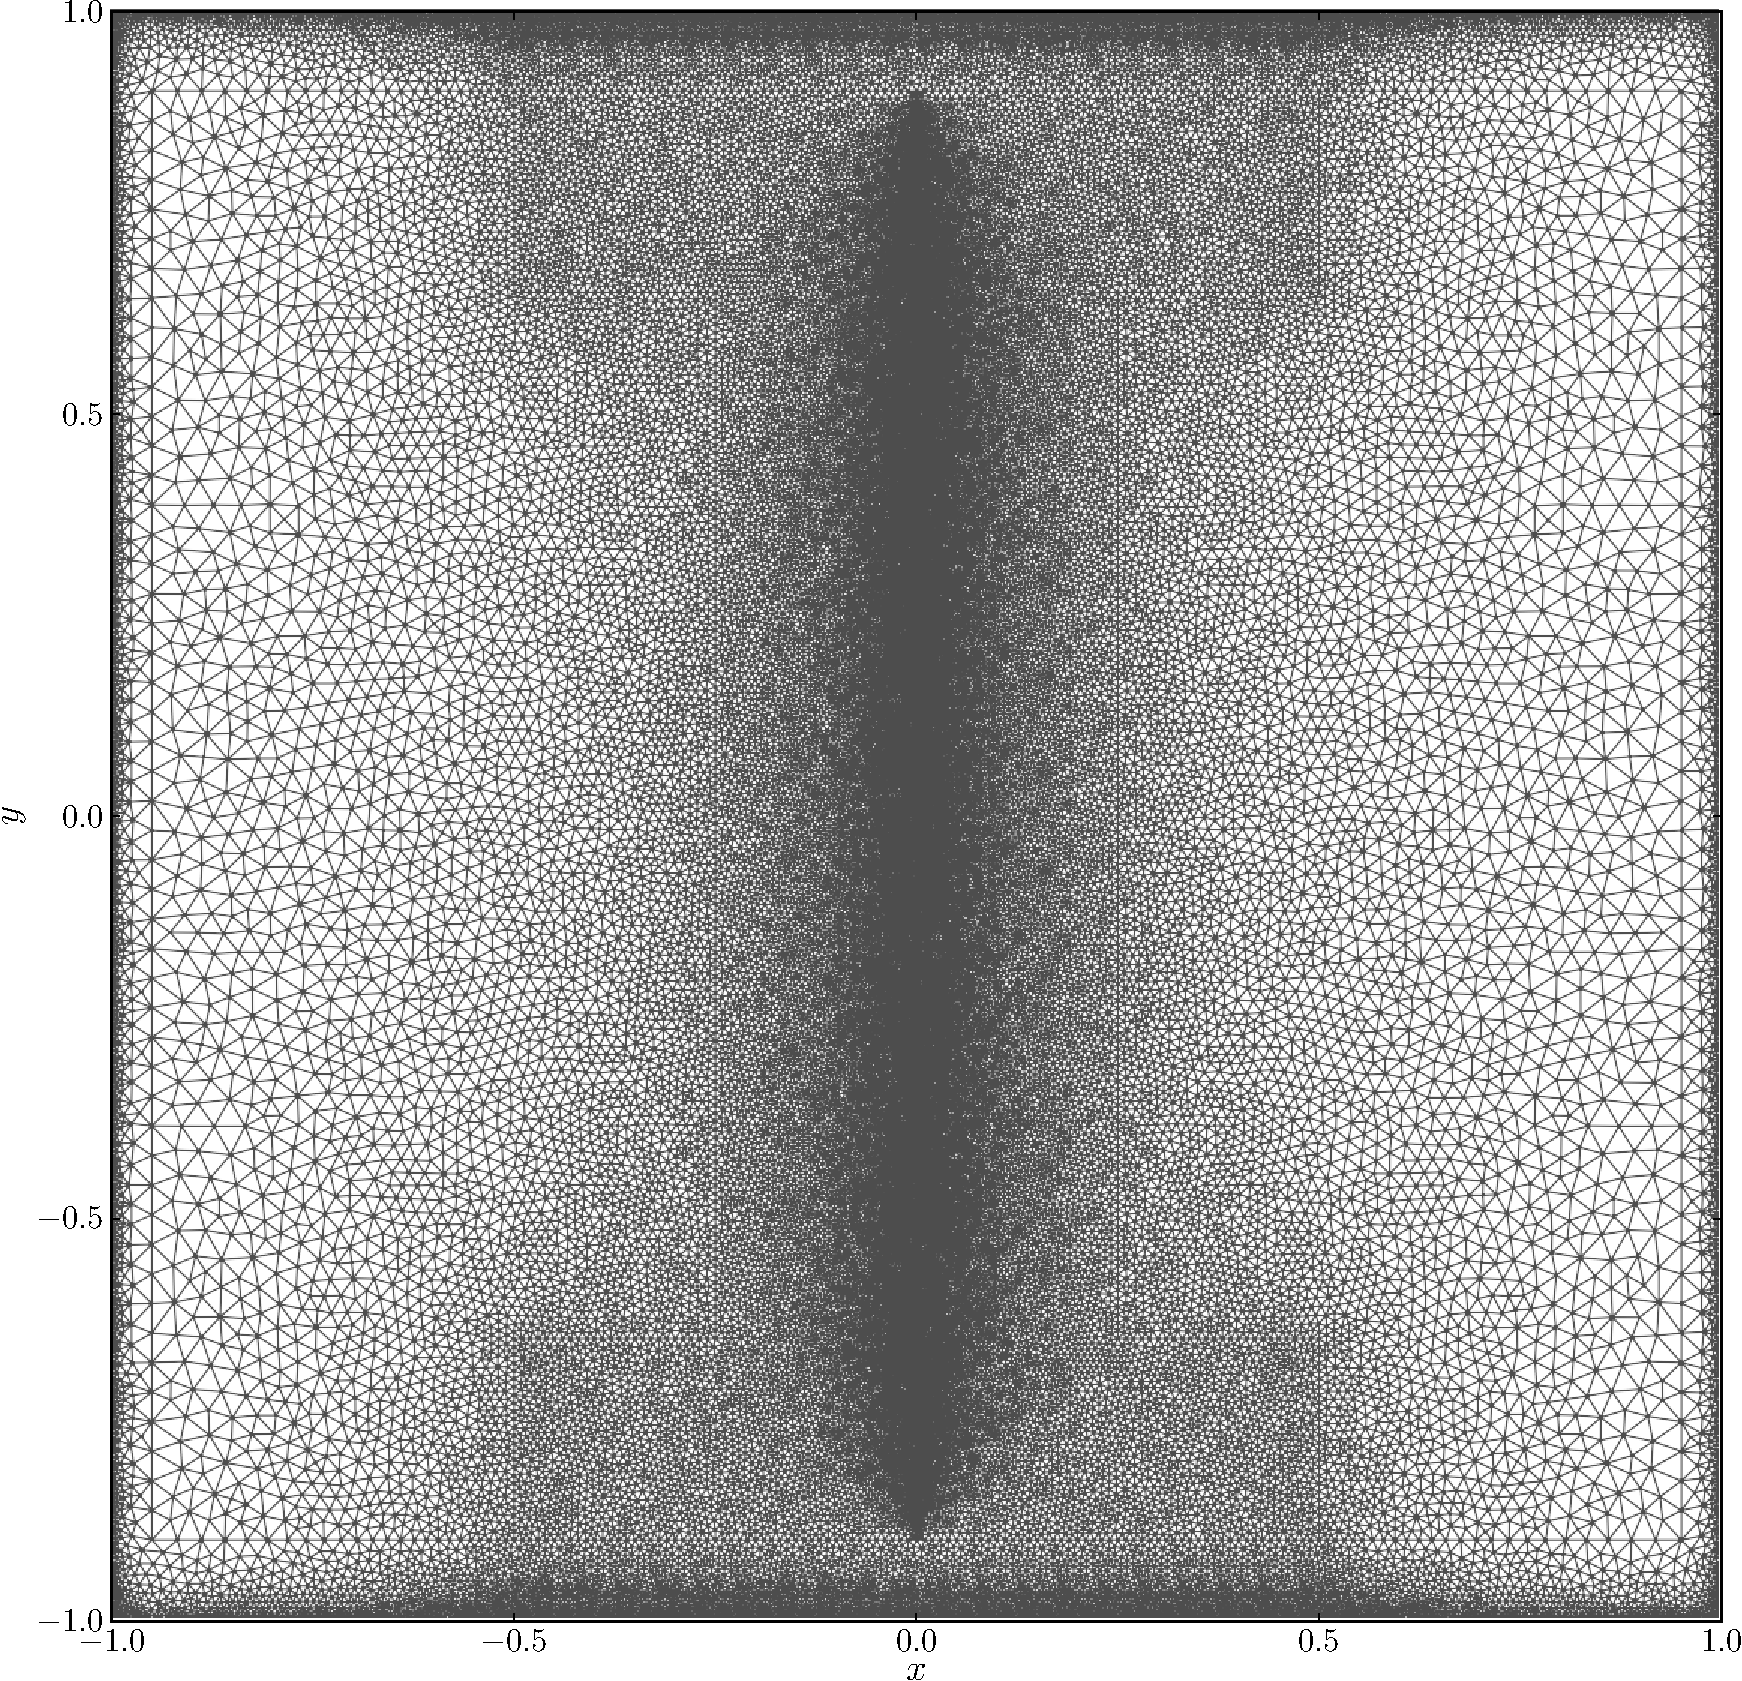
\includegraphics[width=\textwidth]{figures/eulerian/clercxBruneauDomainMesh-crop.pdf}
             \caption{Domain mesh}
             \label{fig:clercxBruneauDomainMesh}
     \end{subfigure}
     \caption{Domain of the Clercx-Bruneau dipole collision problem. The figure depicts \textbf{(a)} the definition of the domain with the fluid domain [gray] and the no-slip boundary [blue]; and \textbf{(b)} the unstructured mesh of the domain with $N_{\mathrm{vert}} = 48k$.}
     \label{fig:clercxBruneauDomain}
	\end{figure}

For this research, we decided to use the simpler case of normal collision at $Re=625$, where $Re$ is the integral-scale Reynolds number defined as,
	\begin{equation}
	Re = \frac{UW}{\nu},
	\end{equation}
where $U$ is the characteristic velocity of the flow, $W$ is half width of domain, and $\nu$ is the kinematic viscosity. We require a low Reynolds number as the Eulerian method solves an incompressible laminar. The domain $\Omega$ of the problem is square with bounds $\Omega = [-1,1]^2$, as shown in figure \ref{fig:clercxBruneauDomainDefinition}. The problem is defined in a closed box, where the Eulerian domain is enclosed in a no-slip boundary $\partial{\Omega}_{\mathrm{wall}}$ where dipole will collide and interact. 

The initial conditions of the Clercx-Bruneau dipole is a smooth vorticity distribution which a positive monopole at $(x_1,y_1)=(0.1,0)$ and the negative monopole at $(x_2,y_2)=(-0.1,0)$, with each having a core radius $R = 0.1$. The vorticity distribution of the combined monopole is given as,
	\begin{equation}
	\begin{split}
	\omega(\mathbf{x},0) = \quad &\hat{\omega}_1\left[1-\left(\frac{r_1}{R}\right)^2\right]\exp\left\{-\left(\frac{r_1}{R}\right)^2\right\} \\
	+\ &\hat{\omega}_2\left[1-\left(\frac{r_2}{R}\right)^2\right]\exp\left\{-\left(\frac{r_1}{R}\right)^2\right\} ,
	\end{split}
	\label{eq:clercxBruneauOmega0}
	\end{equation}
where $\hat{\omega_1} = - \hat{\omega_2} \approx 299.528385375226$ is the extremum vorticity value of the monopole at $r_1=r_2=0$. The radii $r_1$ and $r_2$ are the radial distance from the positive and the negative monopoles respectively. Figure \ref{fig:dipole_contourLine_portrait}a shows the vorticity contours of this initial vorticity distribution. The initial vorticity distribution decays at an exponential rate to zero at the no-slip boundary. This means the no-slip boundary condition is still guaranteed for the initial distribution. To initialize the problem in the Eulerian domain with $\mathbf{u}-p$, we used the velocity distribution, 
	\begin{subequations}
	\begin{align}
	u(\mathbf{x},t) & = -\frac{1}{2}\lvert\hat{\omega}_1\rvert(y-y_1)\exp\left\{-\left(\frac{r_1}{R}\right)^2\right\} + \frac{1}{2}\lvert\hat{\omega}_2\rvert(y-y_2)\exp\left\{-\left(\frac{r_2}{R}\right)^2\right\}, \\
	v(\mathbf{x},t) & = +\frac{1}{2}\lvert\hat{\omega}_1\rvert(x-x_1)\exp\left\{-\left(\frac{r_1}{R}\right)^2\right\} - \frac{1}{2}\lvert\hat{\omega}_2\rvert(x-x_2)\exp\left\{-\left(\frac{r_2}{R}\right)^2\right\},
	\end{align}
	\label{eq:clercxBruneauVel0}
	\end{subequations}
where $u$ and $v$ are the velocity in the $x$ and $y$ direction, respectively. The fluid domain of the Eulerian domain, show in figure \ref{fig:clercxBruneauDomainDefinition} was discretized using an controlled unstructured meshing method. From the velocity distribution, equation \ref{eq:clercxBruneauVel0}, we see that the maximum velocity in the fluid will be along the $y$-axis (i.e $x=0$). Therefore, to satisfy the $CFL$ condition, we need the minimum cell size at the location of the maximum velocity. Furthermore, to ensure the vorticity generation at the no-slip boundary is defined accurately, we increased resolution of the mesh at the boundary. The third region where we increased the resolution is where the dipole and the wall interacts (i.e $-0.5\le{x}\le0.5$ and $0.5\le{\left|y\right|}\le1$). In the region where there is no vorticity, we do not need high resolution (i.e $0.5\le{\left|x\right|}\le1$ and $-0.5\le{y}\le0.5$). With these parameterization, we obtained an unstructured grid with $N_{\mathrm{vert}}=48k$ vertices.

\subsubsection*{Results}
After initializing the velocity field in the discretized domain, the problem was evolved from $t=0$ to $t=2.0$ where $t$ was non-dimensionalized using $W/U$. Using the CFL condition, equation \ref{eq:cfl}, we determine that the simulation required a time step size $\Delta = \num{1.25e-5}$, with a total of $160k$ time steps. Figure \ref{fig:dipole_contourLine_portrait} shows the evolution of the vorticity field at various instances ($t = 0, 0.25, 0.5, 0.75, 1.25$). During the initial stages of the simulation, the initialized dipole travels along the $y$-axis towards the bottom no-slip boundary. The weaker outer regions of the core dipole travels in the opposite direction, and for this simulation, this evolution of the this dipole is ignored. 

The main dipole approaches the bottom boundary, where the no-slip boundary generates vorticity to ensure no-through flow, figure \ref{fig:dipole_contourLine_portrait}b. As the primary dipole approaches closer, the vorticity filament at the wall rolls up and combines with the primary dipole forming two secondary dipoles, that is asymmetric across the $y$-axis. Figure \ref{fig:dipole_contourLine_portrait}c shows the state of the vorticity field at $t=0.5$ after the secondary dipoles are generated. This secondary dipole initially travels away from the bottom wall and later on approaches the wall again, colliding for a second time and creating a tertiary vortex, figure \ref{fig:dipole_contourLine_portrait}d. The dipole stops convecting any further and diffuses as time progresses, as shown for the time instants $t = 1$ and $t = 1.25$.

Figure \ref{fig:vorticity_contour_comparison} compares the vorticity contours in a small part of the computation domain ($0\leqslant x \leqslant 0.6$ and $-1 \leqslant y \leqslant -0.4$) at $t = 1$. The positive vortex (solid black) is surrounded by the negative vortex (dashed black). The primary observation tells us that the overall shape of the vorticity contours is very similar to the reference data. However we see that in the present simulation, more iso-vorticity lines are present meaning that the diffusion of the core is slight different.

	\begin{figure}[p]
	\centering
	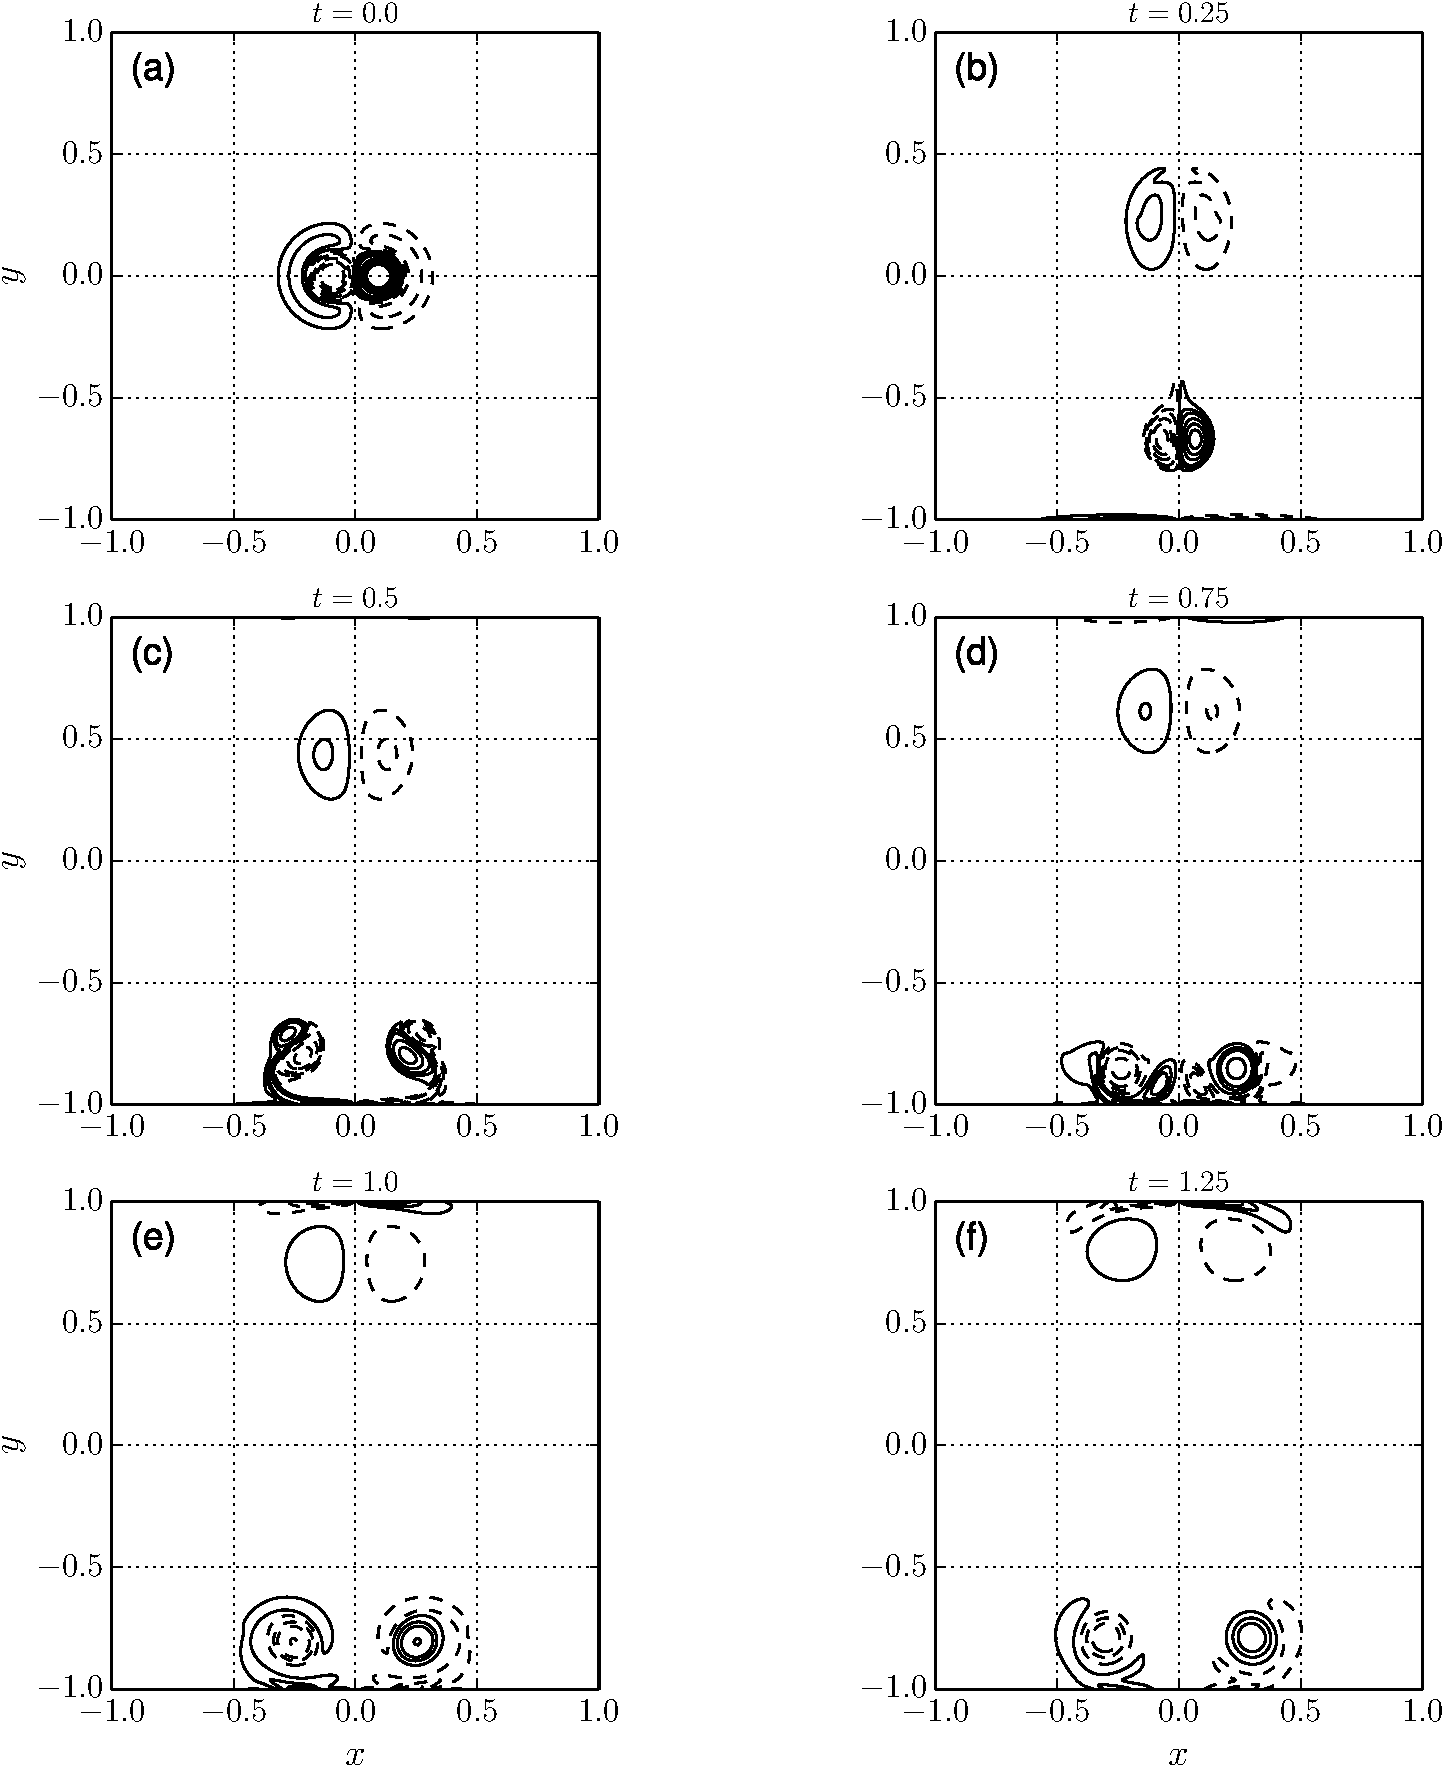
\includegraphics[width=\linewidth]{./figures/eulerian/dipole_contourLine_portrait-crop.pdf}
	\caption{Vorticity contour plots of the normal Clercx-Bruneau dipole-wall collision experiment at $Re=625$ at $t = 0, 0.25, 0.5, 0.75, 1.0, 1.25$ with vorticity contour levels at -320,-200,-100,-50,-10, 10, 50, 100, 200, 320. The figure depicts positive contours [---, solid black], and negative contours [- -, dashed black].}
	\label{fig:dipole_contourLine_portrait}
	\end{figure}
	
	\ctable[
		caption = {Summary of the parameters for the Clercx-Bruneau normal collision of a dipole with a no-slip wall \cite{Clercx2006a}.},
		label   = {tab:clercxBruneauParameters},
		pos = p,]{lcll}{}{\FL
		Parameters					& Value 				& Unit		& Description \ML
		$\Omega$               		& $\left[-1,1\right]^2$ &\si{m}		& Eulerian domain bounds \\
		$Re$  			       		& $625$ 				&-			& Reynolds number \\ 
		$U$			         		& $1$ 					&\si{m.s^{-1}}& Characteristic velocity\\		
		$W$			         		& $1$ 					&\si{m}		& Half width of the domain\\		
		$\nu$						& $\num{1.6e-3}$ 		&\si{kg.s^{-1}.m^{-1}}& Kinematic viscosity\\
		$ (x,y)_{1,2}$				& $(\pm0.1,0)$			& \si{m}    & Initial location of the dipole\\
		$ \hat{\omega}_{1,2}$		& $\pm 299.5283853752226$ & -   	& Maximum vorticity of the monopole\\
		$ (t_0,t_f)$ 		    	& $(0,2)$				& \si{s} 	& Initial and final scaled viscous time\\
		$ \mathrm{CFL}$				& $0.95$ 				& -			& CFL number\\	        	        
		$ \lVert\mathbf{u}\rVert_{\mathrm{max}}$	& $12$	& \si{m.s^{-1}}	& Maximum fluid velocity\\
		$ \Delta t$ 		    	& $\num{1.25e-5}$		& \si{s} 	& Time step size\\
		$ N_{\mathrm{vert}}$ 		& $\sim48k$ 			& -			& Number of mesh vertices\\
		$ h_{\mathrm{min}}$			& $\sim\num{3.6e-3}$ &\si{m}		& Minimum mesh cell size\\	        
		$ N_{\mathrm{tsteps}}$ 		& $160,000$				& -	     	& Number of time integration steps\\
		$\mathrm{ID}_{\mathrm{fluid}}$ & $1$ 				& - 		& Fluid domain I.D\\
		$\mathrm{ID}_{\mathrm{wall}}$ & $2$ 				& - 		& No-slip boundary I.D\LL}
	
	\begin{figure}[p]
     \centering
     \begin{subfigure}[t]{0.4\textwidth}
             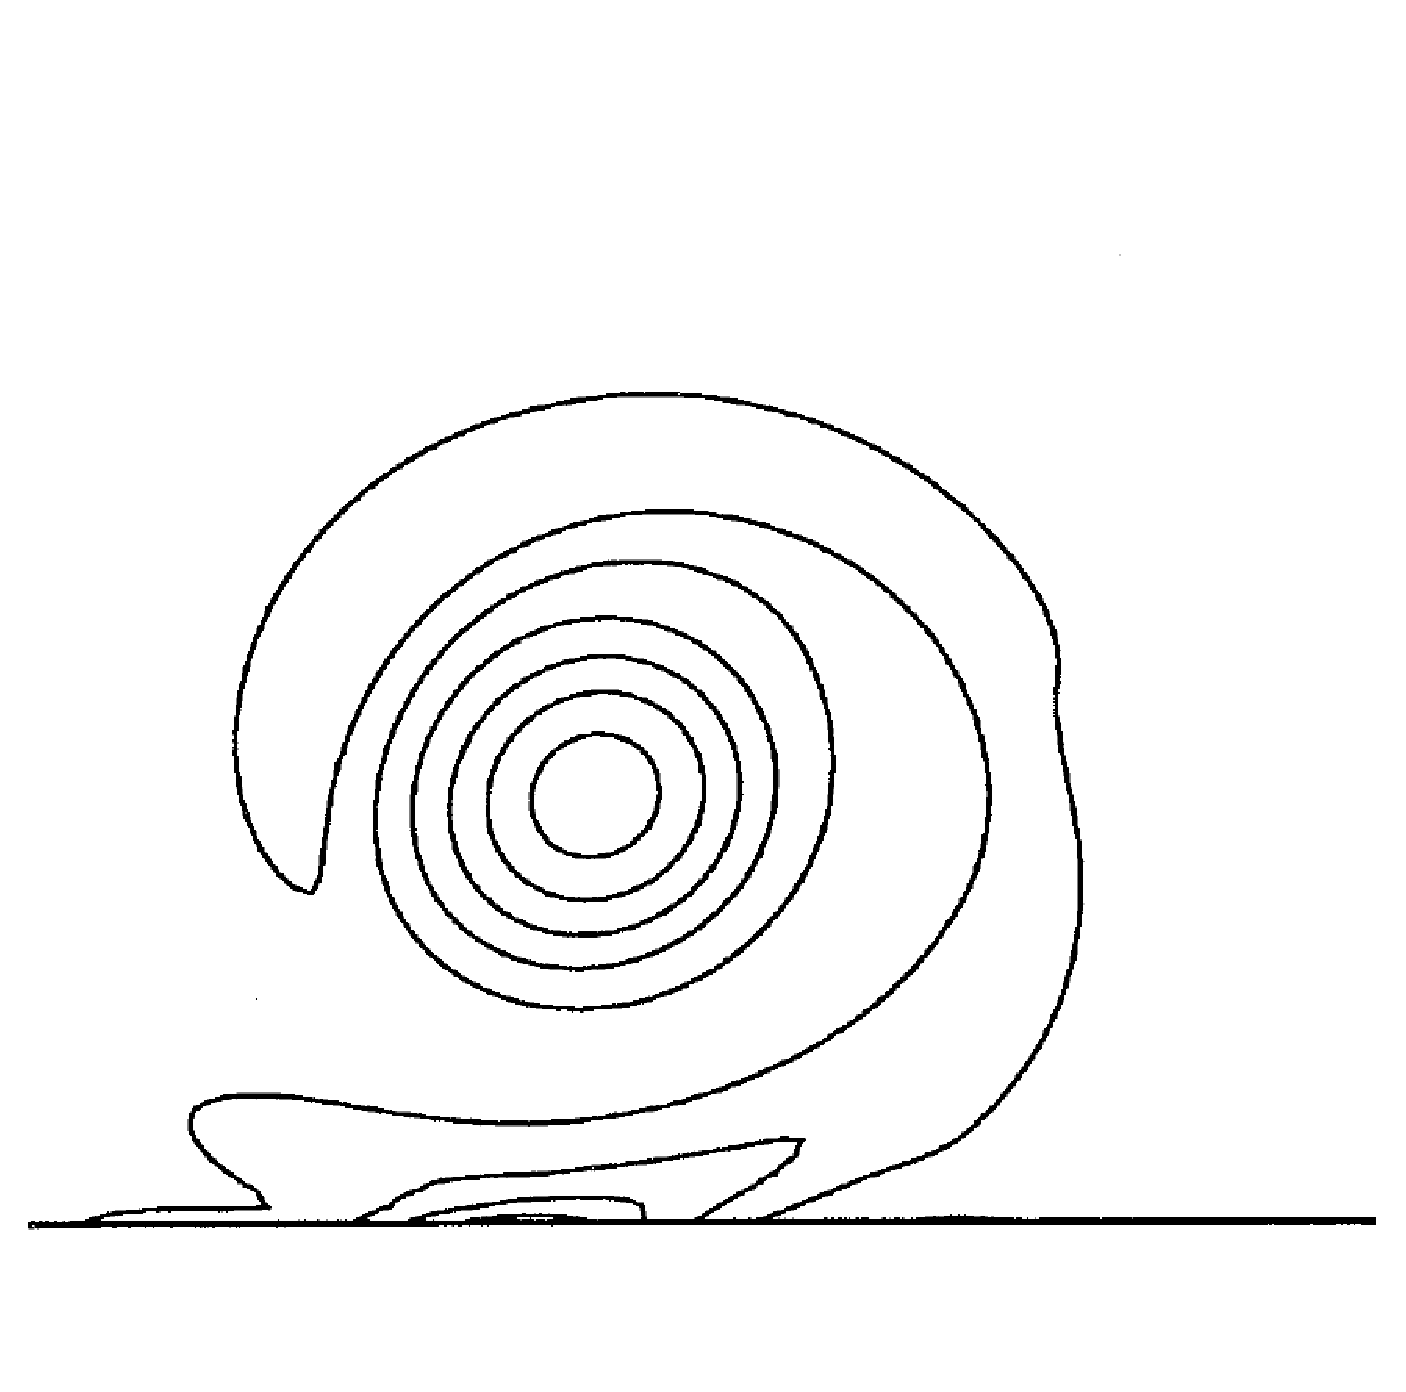
\includegraphics[width=\textwidth]{figures/eulerian/VorticityContourPlot-rotated270.pdf}
             \caption{Literature}
             \label{fig:VorticityContourPlot}
     \end{subfigure}%
     ~ %add desired spacing between images, e. g. ~, \quad, \qquad etc.
       %(or a blank line to force the subfigure onto a new line)
     \begin{subfigure}[t]{0.5\textwidth}
             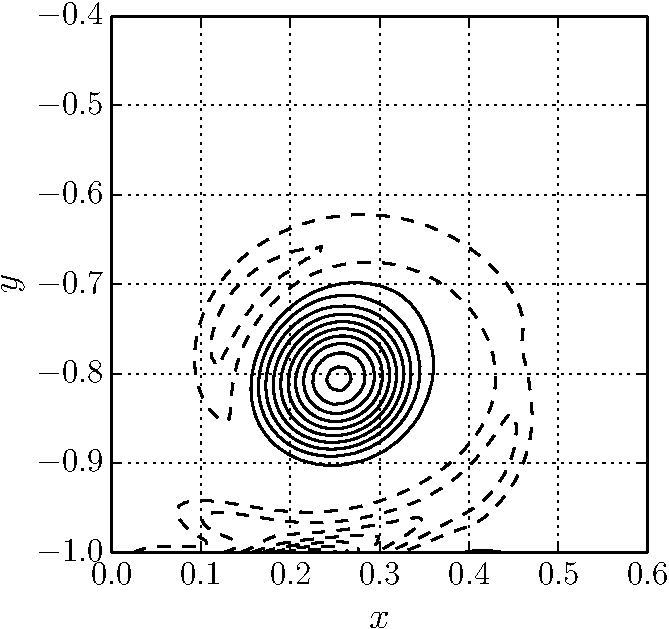
\includegraphics[width=\textwidth]{figures/eulerian/dipole_contourLine_t1p0-crop.pdf}
             \caption{Present study}
             \label{fig:dipole_contourLine_t1p0}
     \end{subfigure}
     \caption{Comparison of the vorticity contours at $t=1$. The figure compares the plot obtained by \textbf{(a)} literature and \textbf{(b)} the present study.}
     \label{fig:vorticity_contour_comparison}
	\end{figure}	
	
To determine the variation of the fluid properties as the time progresses, Clercx \& Bruneau investigated the evolution of the total kinetic energy $E(t)$, the total enstrophy $\Omega(T)$, and the total Palinstrophy $P(t)$ of the flow field. The total kinetic energy $E(t)$ of the dipolar field can be determined as,
	\begin{equation}
	E(t) = \frac{1}{2} \int\int \mathbf{u}^2(\mathbf{x},t)\ \mathrm{d}x\mathrm{d}y,
	\end{equation}
and at $t=0$, $E(0) = 2$. The total enstrophy of the flow is determined as, 
	\begin{equation}
	\Omega(t) = \frac{1}{2}\int\int\omega^2(\mathbf{x},t)\ \mathrm{d}x\mathrm{d}y,
	\end{equation}	
and can seen as the energy of the vorticity. The change in enstrophy of the field can give an insight to dissipation rate in the fluid. At $t=0$, the enstrophy of the fluid is $\Omega(0)=800$. The total Palinstrophy $P(t)$ of the flow measures the gradient of the vorticity, 
	\begin{equation}
	P(t) = \frac{1}{2}\int\int\left[\nabla\omega(\mathbf{x},t)\right]^2\ \mathrm{d}x\mathrm{d}y,
	\end{equation}
and gives an insight to generation of vorticity at the no-slip boundary. Figure \ref{fig:dipole_comparison} compare the evolution of these time dependent parameters with the reference data provided by Clercx \& Bruneau (dotted red) for $t=0.25$, $t=0.5$ and $t=0.75$. The kinetic energy, figure \ref{fig:dipole_KineticEnergy_comparison}, reduced from $E(0) = 2$ to $E(2) \approx 0.3$. At $t=0.4$, we have small kink representing the approach of the primary dipole at the wall. When plotting the reference data, we see that the variation in kinetic energy matches perfectly at $t=0.25$, $t=0.5$ and $t=0.75$.
	
	\begin{figure}[p]
     \centering
     \begin{subfigure}[t]{0.49\textwidth}
             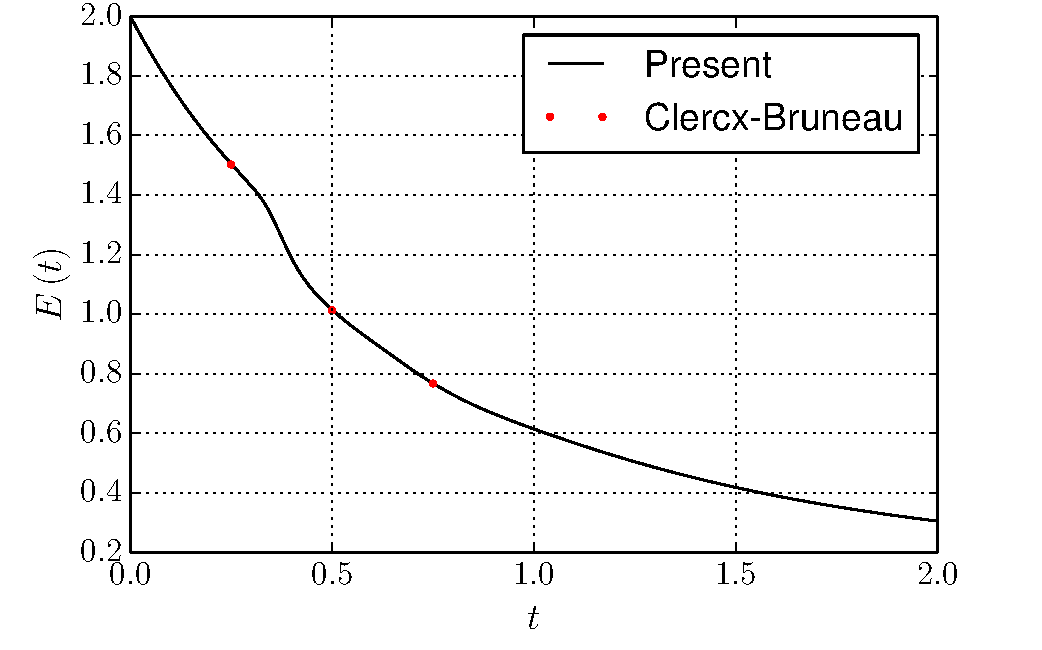
\includegraphics[width=\textwidth]{figures/eulerian/dipole_KineticEnergy_comparison.pdf}
             \caption{Kinetic Energy $E(t)$}
             \label{fig:dipole_KineticEnergy_comparison}
     \end{subfigure}%
     ~ %add desired spacing between images, e. g. ~, \quad, \qquad etc.
       %(or a blank line to force the subfigure onto a new line)
     \begin{subfigure}[t]{0.49\textwidth}
             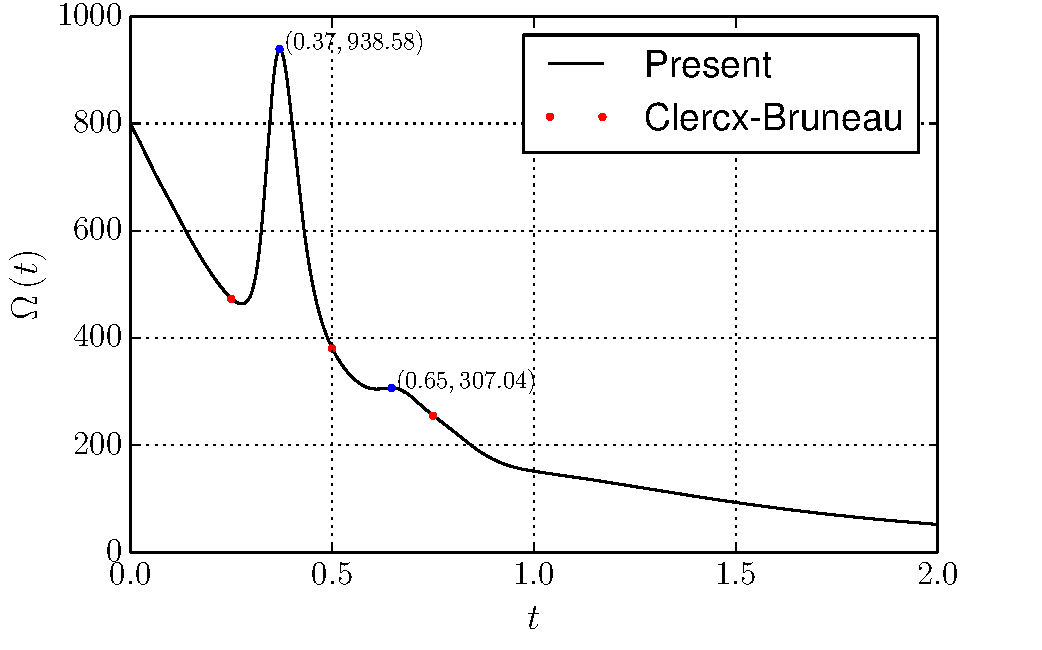
\includegraphics[width=\textwidth]{figures/eulerian/dipole_Enstrophy_comparison.pdf}
             \caption{Enstrophy $\Omega(t)$}
             \label{fig:dipole_Enstrophy_comparison}
     \end{subfigure}
     
     \begin{subfigure}[b]{0.49\textwidth}
             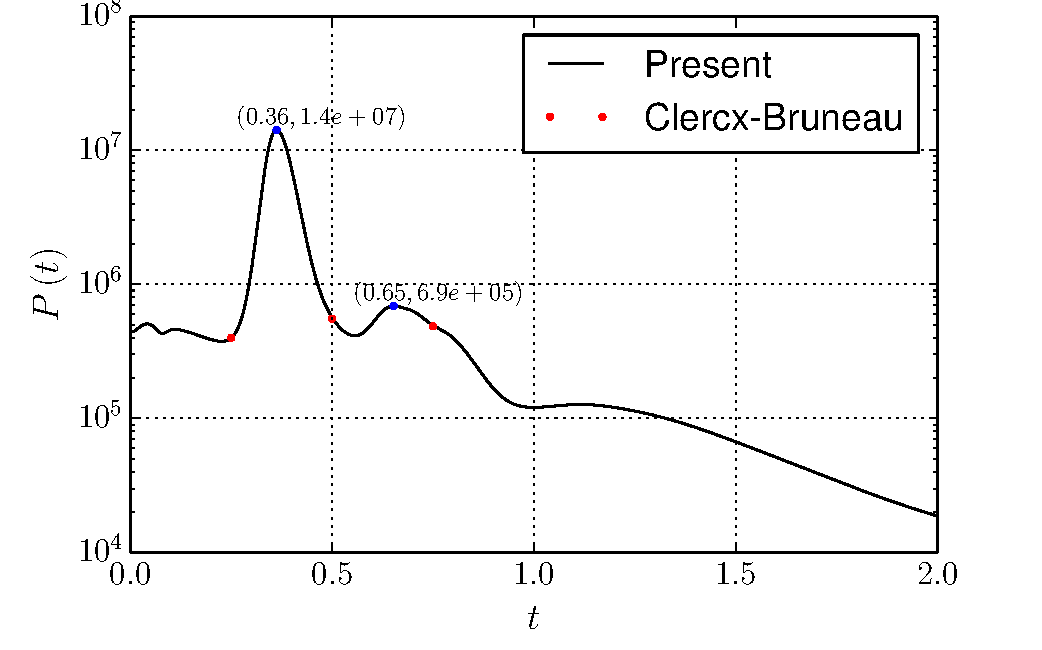
\includegraphics[width=\textwidth]{figures/eulerian/dipole_Palinstrophy_comparison.pdf}
             \caption{Palinstrophy $P(t)$}
             \label{fig:dipole_Palinstrophy_comparison}
     \end{subfigure}
     ~
     \begin{subfigure}[b]{0.48\textwidth}
		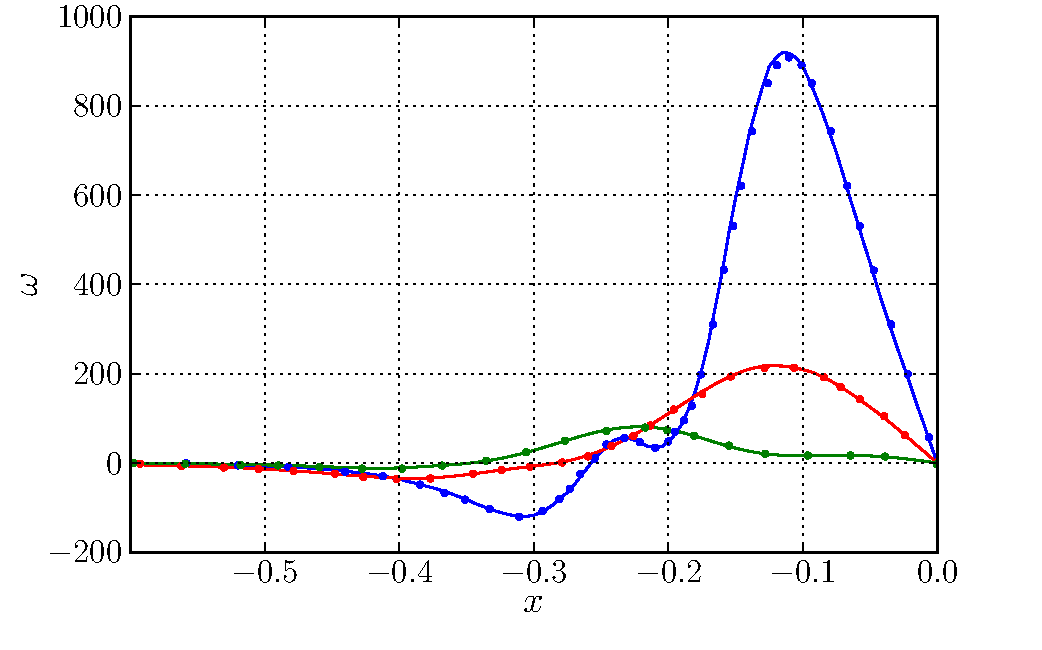
\includegraphics[width=\textwidth]{./figures/eulerian/VorticityAtBoundary.pdf}
		\caption{Vorticity at the boundary y = -1.}
		\label{fig:VorticityAtBoundary}
     \end{subfigure}     
     
     \caption{Comparison of the fluid parameters. Figure \textbf{(a)}, \textbf{(b)}, \textbf{(c)} compares the evolution of the fluid properties from $t=0$ to $t=2$. Figure \textbf{d} compares the vorticity generated at the bottom-left wall ($y=-1$, $-0.6\leqslant x \leqslant 0$) at $t=0.4$ [{\color{plotBlue}{---}}, solid blue], $t=0.6$ [{\color{plotRed}{---}}, solid red] and $t=1$ [{\color{plotGreen}{---}}, solid green].}
     \label{fig:dipole_comparison}
	\end{figure}


	\ctable[
	    caption = {A summary of the values of the first two maxima of the enstrophy $E$ and palinstrophy $P$ occurring at $t_1$ and $t_2$ respectively.},
	    label   = {tab:euleriandipoleCollisionComparison},
	    maxwidth = \textwidth,
	    pos = p,
	]{ccrrrr}{\tnote{Data obtained from Clercx \& Bruneau \cite{Clercx2006a}}}{\FL
	\multirow{2}{*}{Instant} & 	\multirow{2}{*}{Case} & \multicolumn{2}{c}{Enstrophy $\Omega$} & \multicolumn{2}{c}{Palinstrophy $P$}\\
	\noalign{\smallskip}\cline{3-6}\noalign{\smallskip}
			& 			& $t$ & $\Omega$ 	& $t$ & $P$\ML
	\multirow{2}{*}{$t_1$} 	& Reference\tmark[a] 	& 0.371 & 933.6 	& 0.361 & $1.39\times10^7$\\
							& Present 		& 0.370 & 938.6 	& 0.360 & $1.40\times10^7$\\
	\multirow{2}{*}{$t_2$} 	& Reference\tmark[a] 	& 0.648 & 305.2 	& 0.652 & $6.78\times10^{5}$\\
							& Present 		& 0.650 & 307.0		& 0.650 & $6.90\times10^{5}$\LL}


Figure \ref{fig:dipole_Enstrophy_comparison} compares the variation in enstrophy ($\Omega$). During the initial stages, the enstrophy decreases linearly, and at $t=0.37$ there is sharp increase in the total enstrophy of the flow $\Omega(0.37) = 938.58$. This indicates the initial impact of dipole with the no-slip wall. After the impact, the enstrophy quickly drops and peaks again at $t=0.65$ reaching $\Omega = 307.04$. In addition, to the 3 data points, Clercx \& Bruneau determined the peak enstrophy of flow. Table \ref{tab:euleriandipoleCollisionComparison} compares the difference between the present study and literature and we see that there is maximum of $0.3\%$ error in time $t$ and $0.6\%$ error in enstrophy $\Omega$. Therefore, the variation in enstrophy is well represented by our Eulerian method.

Figure \ref{fig:dipole_Palinstrophy_comparison} compares the variation in palinstrophy $P(t)$. Similar to enstrophy, we can observe to peak regions at $t=0.36$ and $t=0.65$, respesenting the two collision of the dipole. During the collision, vorticity is generated from the wall to ensure no-through boundary condition, which results in a sharp increase in the gradient of the vorticity. Table \ref{tab:euleriandipoleCollisionComparison} compares the difference with the addition data provided and we see that there is a maximum error of $0.3\%$ in time $t$ and $1.8\%$ in palinstrophy $P$. This is an acceptable error and tells us the generation of vorticity in Eulerian method performs according to theory.
	
Figure \ref{fig:VorticityAtBoundary} compares the vorticity along the boundary of the domain at $y=-1$ for $-0.6 \leqslant x \leqslant 0$. The solid lines represents the present data, and is compared with the dotted data obtained from the reference. The comparison is done for various time instances $t=0.4$, $t=0.6$ and $t=1.0$ and we can finally validate that the Eulerian method accurately represents vorticity generation from the wall.

\subsection{Impulsively started cylinder at $Re=550$}

Finally, we investigated the problem of an impulsively started cylinder at $Re=550$. This validation test ensured that at the end of the simulation, we are able to determine correct forces acting on the body. 

\subsubsection*{Problem Definition}
The \indexAcron{Impulsively Started Cylinder}{ISC} test case simulates the flow around a cylinder exposed to an impulsively started free-stream flow. The test cases focuses on the unsteady behavior of the separated flow past the cylinder. Various experimental and numerical investigation have been performed investigating the flow characterstics, and for this project we relied on the widely used and validated results of Koumoutsakos \& Leonard \cite{Koumoutsakos1995a}. They investigated the flow around the ISC using vortex methods, and provided extensive data on the vorticity profile behind the cylinder and the evolution of the Lift and Drag.

Figure \ref{fig:ISCDomain} shows the domain definition of the ISC problem. Figure \ref{fig:ISCDomainDefinition-crop} shows the fluid domain $\Omega_E$ with an initial conditions $\mathbf{u}=0$, and $p=0$. The domain has the following boundary conditions: the no-slip wall boundary condition at $\partial \Omega_{\mathrm{wall}}$ (solid blue) $\mathbf{u}=0$, the free-stream Dirichlet velocity boundary condition at $\partial \Omega_{\mathrm{dirichlet}}$ (solid red) $\mathbf{u}_{\infty} = [1,0]$, and the pressure outlet $\partial \Omega_{\mathrm{pressure}}$ (solid green). Unlike the previous test cases we now require a pressure outlet boundary condition $\partial p/ \partial \mathbf{n} = 0$, as the velocity field behind the cylinder perturbed and therefore free-stream boundary condition cannot be applied there.

The unsteady simulation has Reynolds number $Re$ of the flow dependent on the diameter of the cylinder $D$,
	\begin{equation}
	Re = \frac{UD}{\nu},
	\end{equation}
and the time $t$ is non-dimensionalized with the radius $R$ of the cylinder,
	\begin{equation}
	T = \frac{U}{R}t.
	\end{equation}
The domain was discretized with $N_{\mathrm{vert}}=48$, with the highest mesh resolutions at the surface of the body, and right behind the body, figure \ref{fig:ISC_mesh} and figure \ref{fig:ISC_mesh_surface}. The simulation was time marched with $\Delta t = \num{1e-3}$ satisfying the CFL condition. The parameter of the simulation are tabulated in table \ref{tab:ISCParameters}.

	\begin{figure}[p]
     \centering
     \begin{subfigure}[t]{0.45\textwidth}
             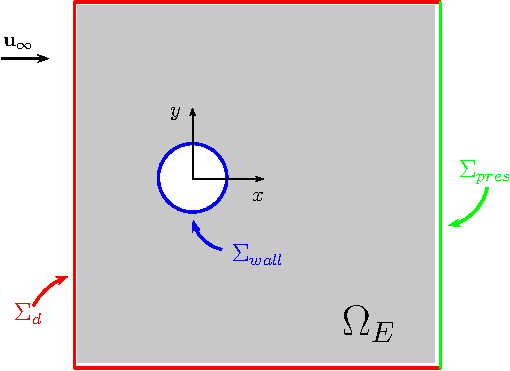
\includegraphics[width=\textwidth]{figures/eulerian/ISCDomainDefinition-crop.pdf}
             \caption{Domain definition}
             \label{fig:ISCDomainDefinition-crop}
     \end{subfigure}%
     ~ %add desired spacing between images, e. g. ~, \quad, \qquad etc.
       %(or a blank line to force the subfigure onto a new line)
     \begin{subfigure}[t]{0.45\textwidth}
             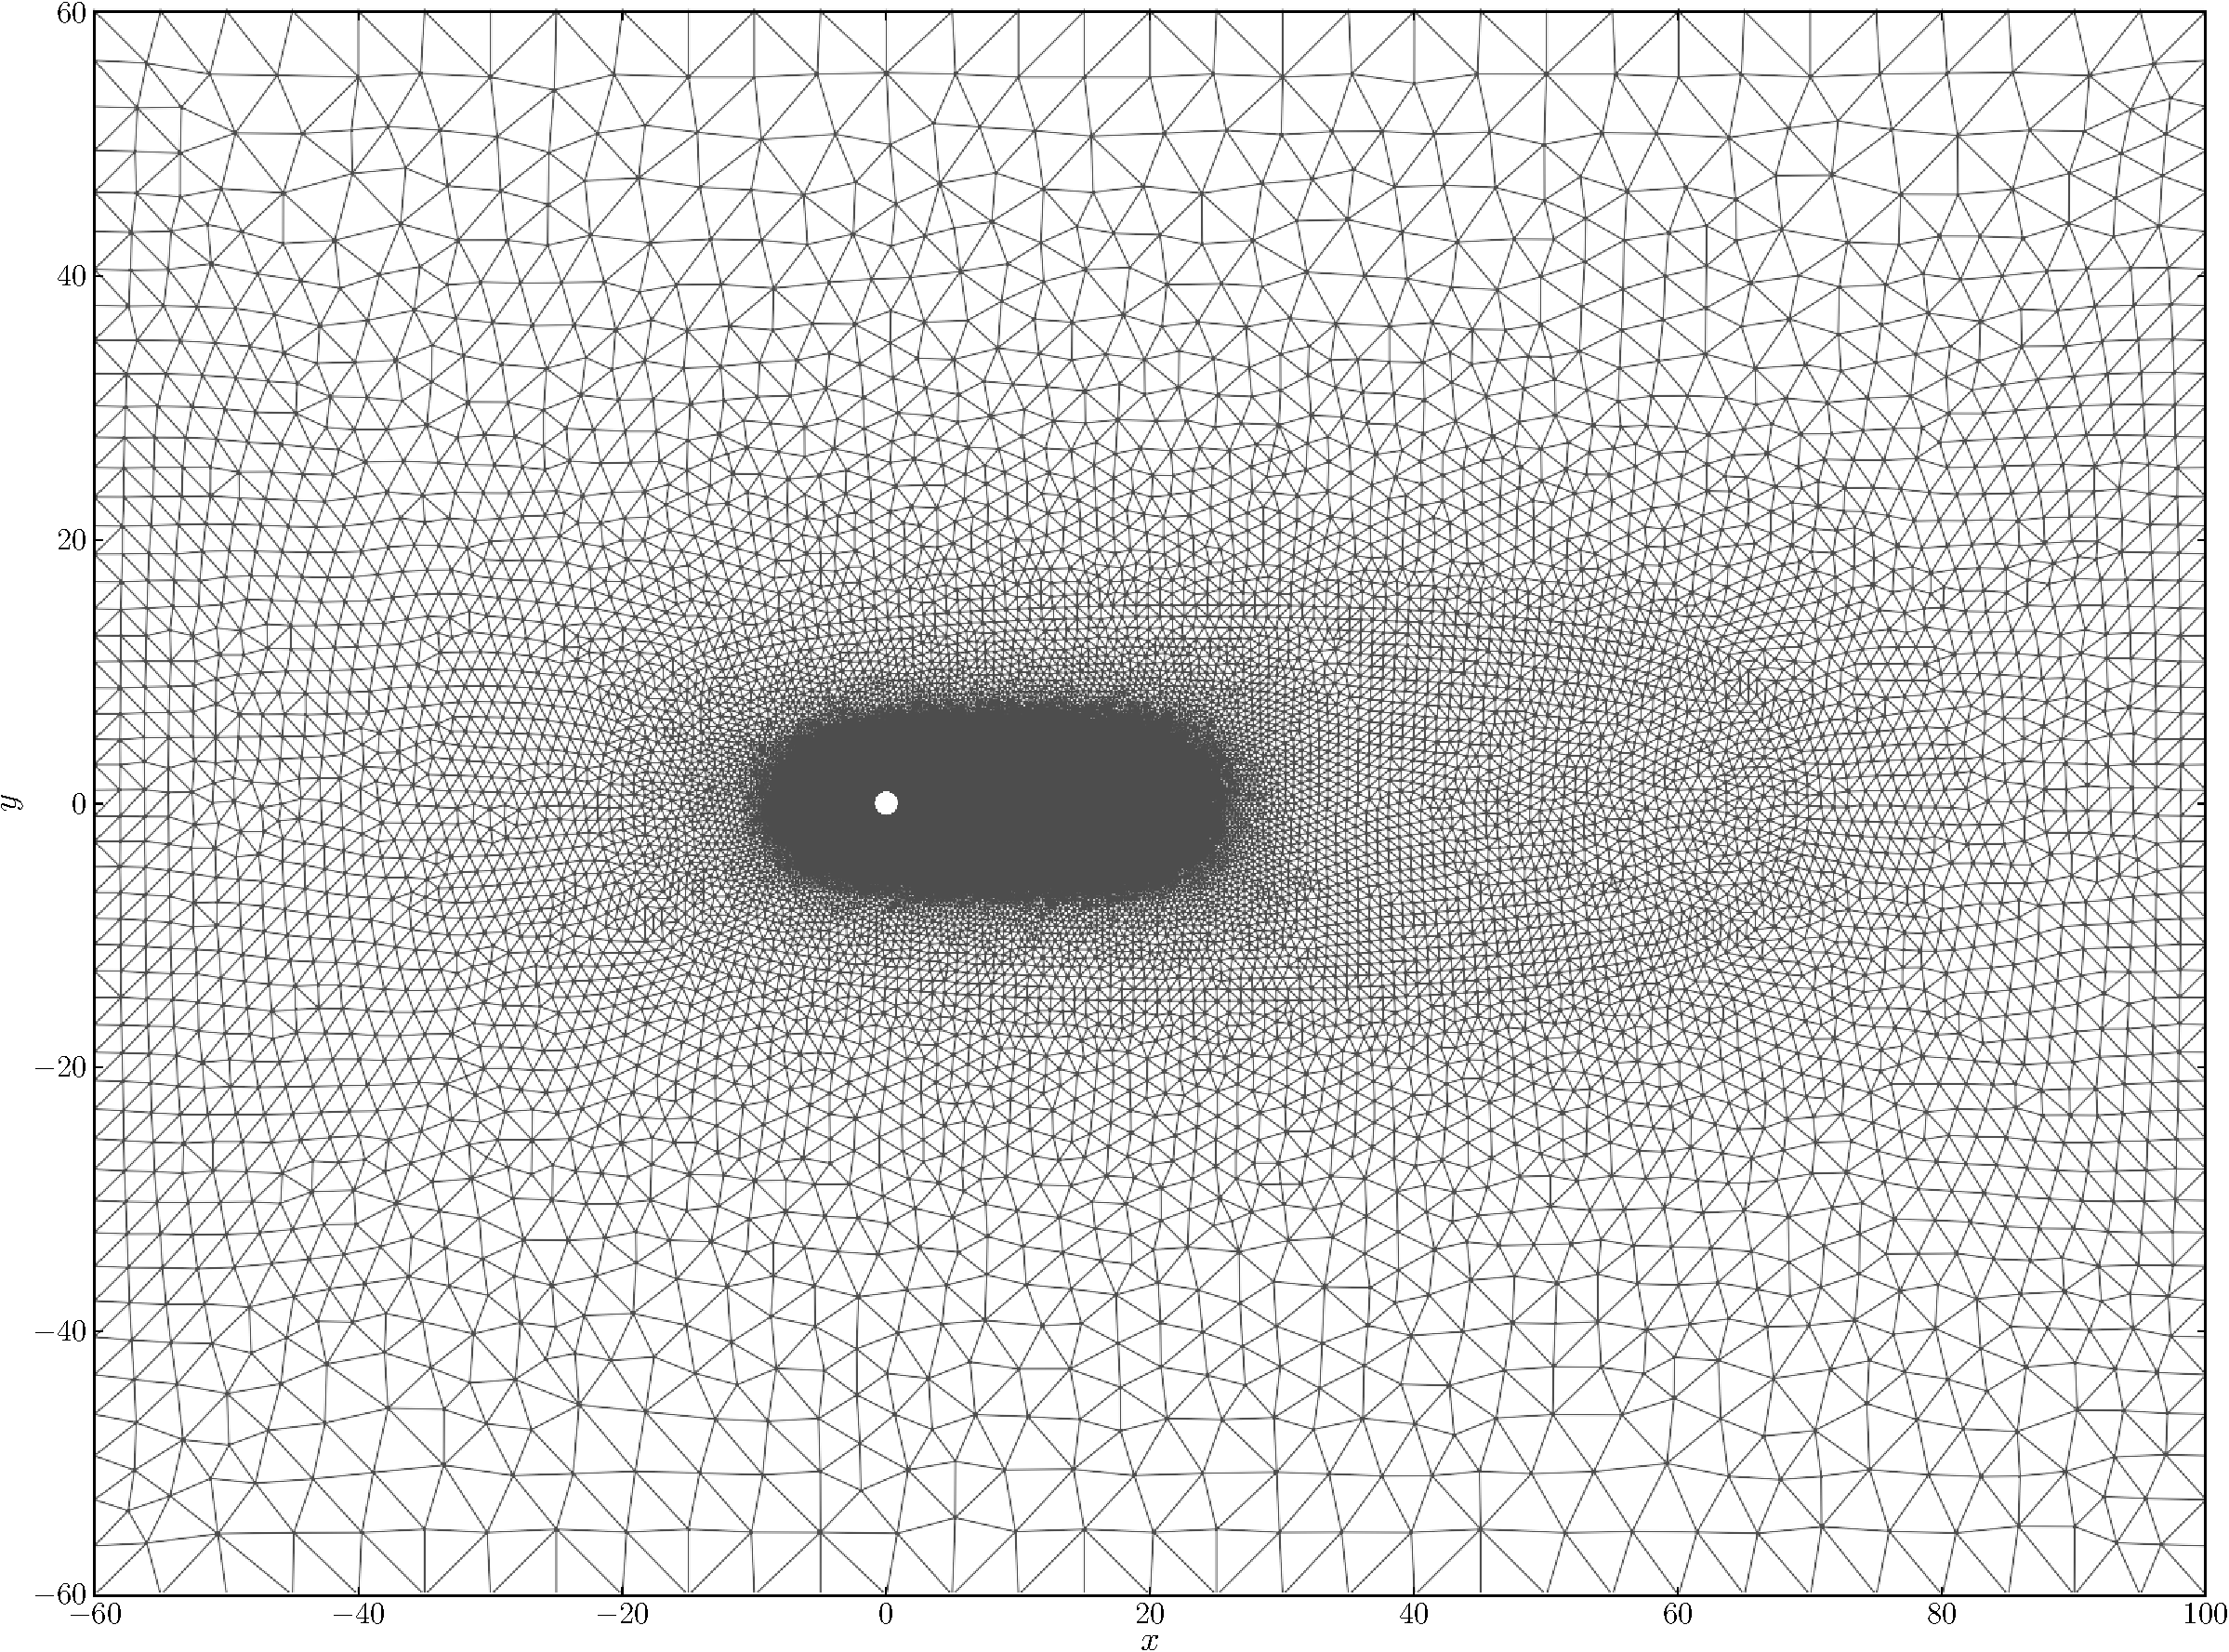
\includegraphics[width=\textwidth]{figures/eulerian/ISC_mesh-crop.pdf}
             \caption{Full mesh}
             \label{fig:ISC_mesh}
     \end{subfigure}

     \begin{subfigure}[t]{0.3\textwidth}
             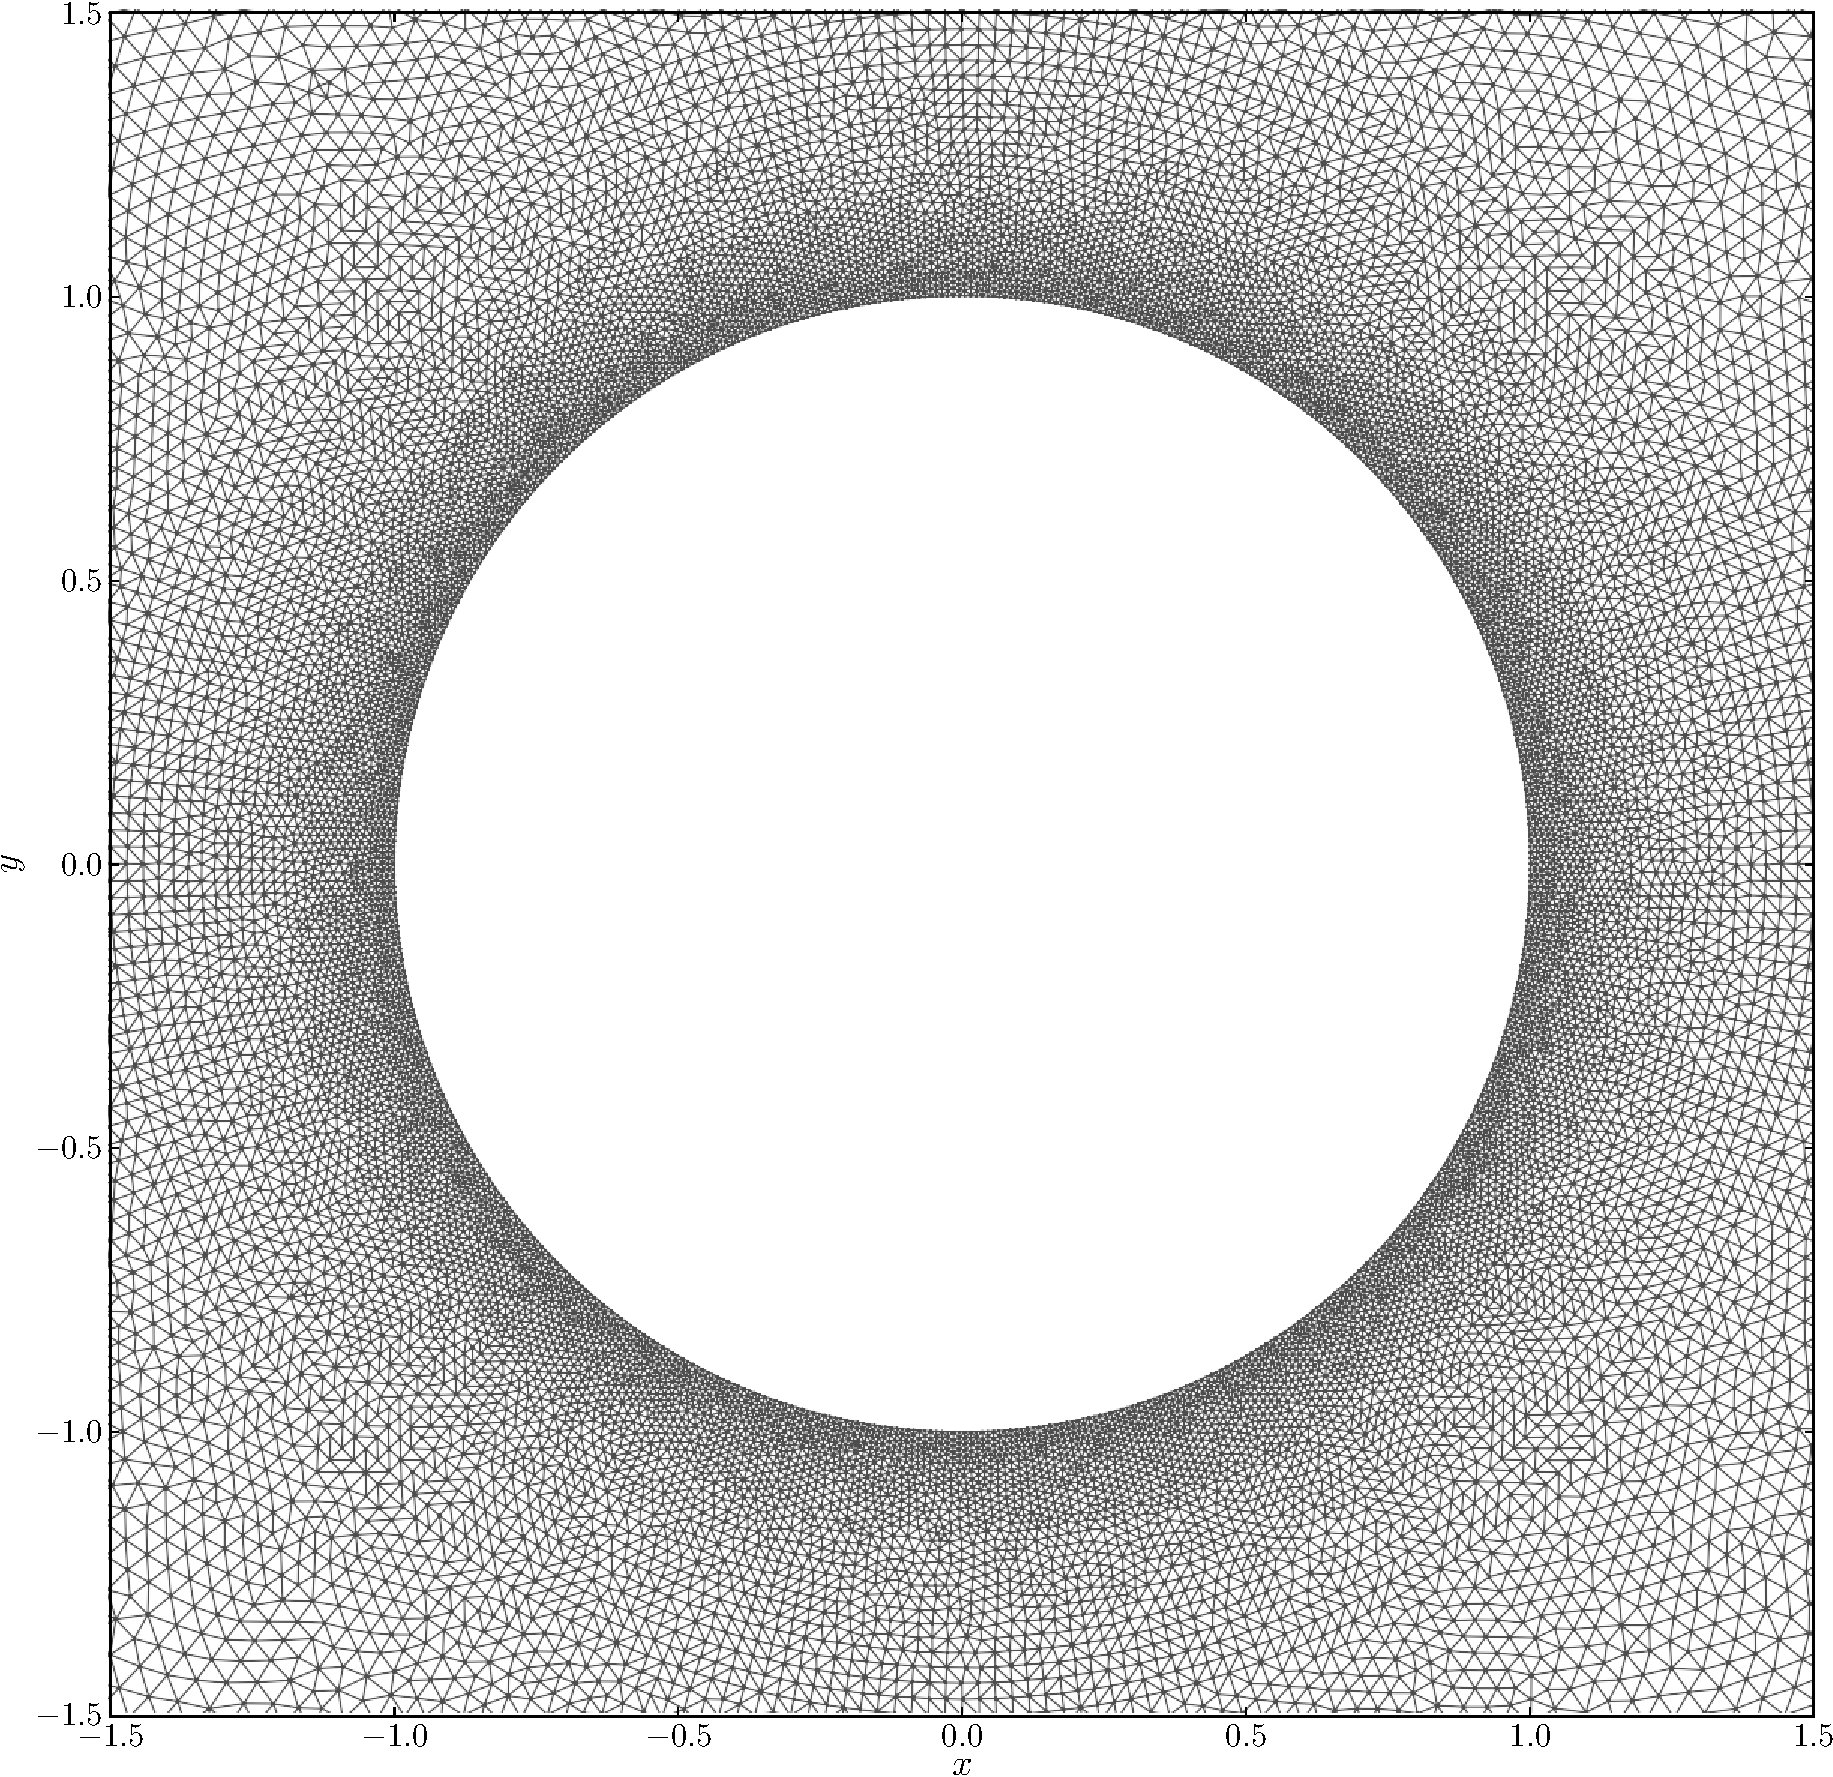
\includegraphics[width=\textwidth]{figures/eulerian/ISC_mesh_surface-crop.pdf}
             \caption{Mesh near the surface}
             \label{fig:ISC_mesh_surface}
     \end{subfigure}

     \caption{Domain of the ISC problem. The figure depicts \textbf{(a)} the definition, \textbf{(b)} the full domain mesh, and \textbf{(c)} the mesh near the surface.}
     \label{fig:ISCDomain}
	\end{figure}

	\ctable[
		caption = {Summary of the parameters for the Impulsively started cylinder test case for $Re=550$.},
		label   = {tab:ISCParameters},
		pos = p,]{lcll}{}{\FL
		Parameters					& Value 				& Unit		& Description \ML
		$\Omega$               		& $\left[-60,100\right]\times[-60,60]$ &\si{m}		& Eulerian domain bounds \\
		$Re$  			       		& $550$ 				&-			& Reynolds number \\ 
		$\mathbf{u}_{\infty}$		& $[1,0]$ 				&\si{m.s^{-1}}& Free-stream velocity\\		
		$R$			         		& $1$ 					&\si{m}		& Radius of cylinder\\		
		$D$			         		& $2$ 					&\si{m}		& Diameter of cylinder\\		
		$\nu$						& $\num{3.6e-3}$ 		&\si{kg.s^{-1}.m^{-1}}& Kinematic viscosity\\
		$ (t_0,t_f)$ 		    	& $(0,100)$				& \si{s} 	& Initial and final non-dimensional time\\
		$ \mathrm{CFL}$				& $0.95$ 				& -			& CFL number\\	        	        
		$ \lVert\mathbf{u}\rVert_{\mathrm{max}}$	& $2.5$	& \si{m.s^{-1}}	& Maximum fluid velocity\\
		$ \Delta t$ 		    	& $\num{1e-3}$		& \si{s} 	& Time step size\\
		$ N_{\mathrm{vert}}$ 		& $\sim47k$ 			& -			& Number of mesh vertices\\
		$ h_{\mathrm{min}}$			& $\sim\num{9.7e-3}$ &\si{m}		& Minimum mesh cell size\\	        
		$ N_{\mathrm{tsteps}}$ 		& $100,000$				& -	     	& Number of time integration steps\\
		$\mathrm{ID}_{\mathrm{fluid}}$ & $1$ 				& - 		& Fluid domain I.D (gray)\\
		$\mathrm{ID}_{\mathrm{wall}}$ & $2$ 				& - 		& No-slip boundary I.D (blue)\\
		$\mathrm{ID}_{\mathrm{dirichlet}}$ & $3$ 			& - 		& Dirichlet boundary I.D (red)\\
		$\mathrm{ID}_{\mathrm{pressure}}$ & $4$ 			& - 		& Pressure boundary I.D (green)\LL}


	\begin{figure}[p]
     \centering
     \begin{subfigure}[t]{0.45\textwidth}
             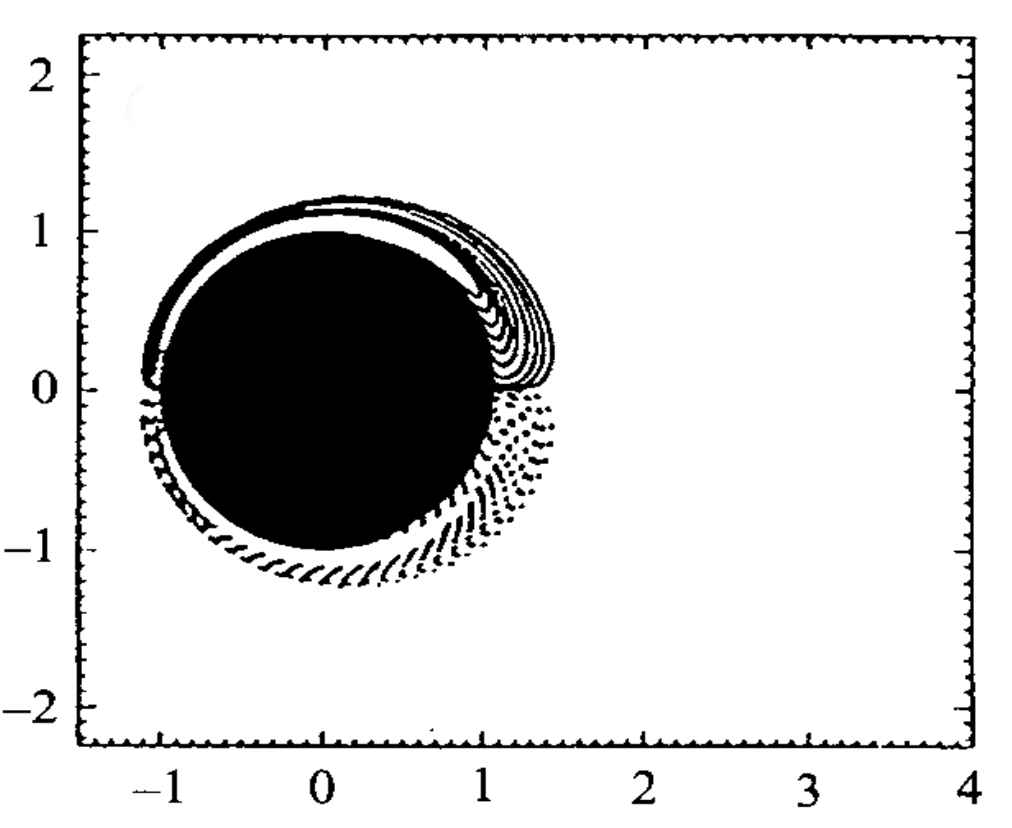
\includegraphics[height=0.2\textheight]{figures/eulerian/ISC_vorticityContours_t1_ref-mod.png}
             \caption{$t=1$ Reference}
             \label{fig:ISC_vorticityContours_t1_ref}
     \end{subfigure}%
     ~ %add desired spacing between images, e. g. ~, \quad, \qquad etc.
       %(or a blank line to force the subfigure onto a new line)
     \begin{subfigure}[t]{0.45\textwidth}
             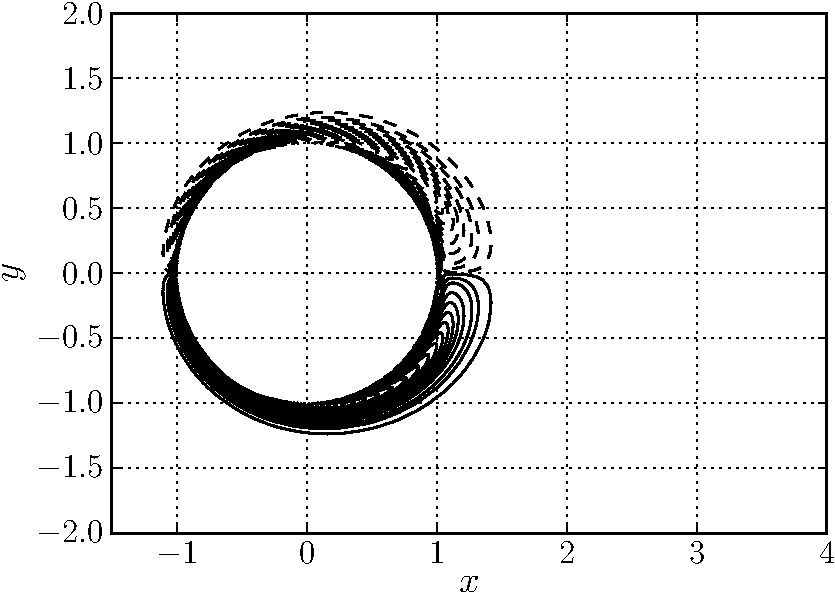
\includegraphics[height=0.2\textheight]{figures/eulerian/ISC_vorticityContours_t1-crop.pdf}
             \caption{$t=1$ Present}
             \label{fig:ISC_vorticityContours_t1-crop}
     \end{subfigure}
     
     \begin{subfigure}[t]{0.45\textwidth}
             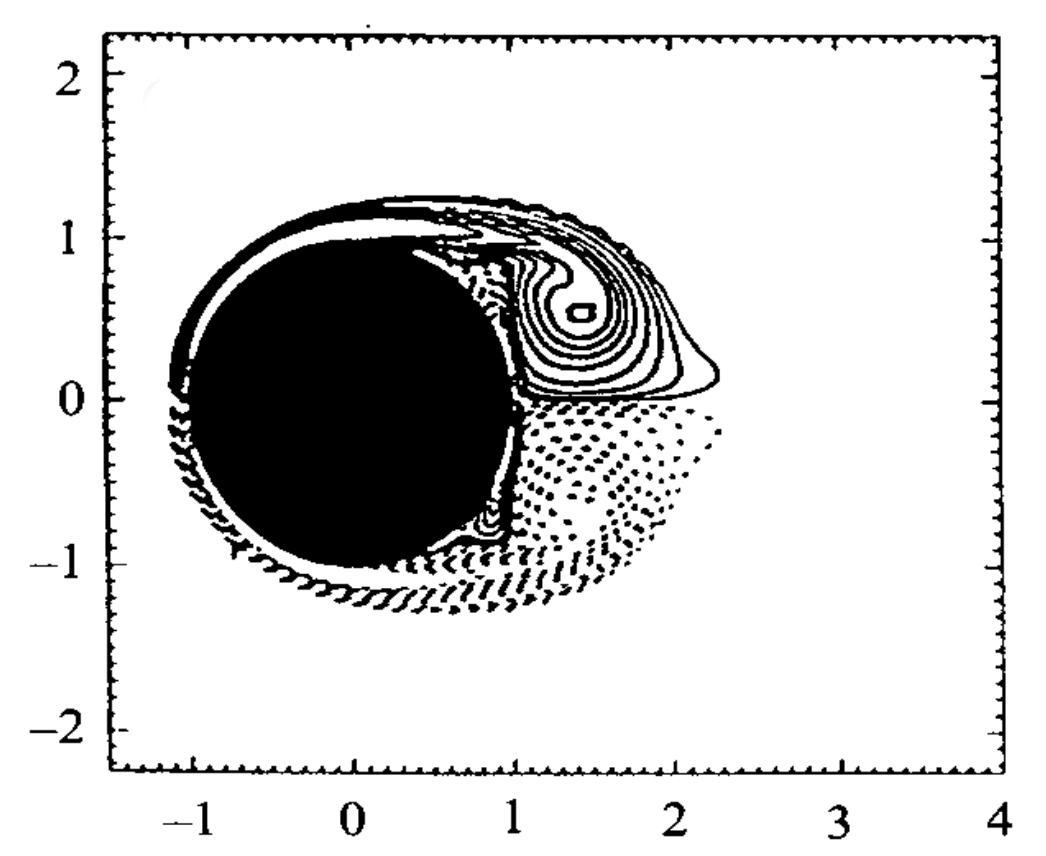
\includegraphics[height=0.2\textheight]{figures/eulerian/ISC_vorticityContours_t3_ref-mod.png}
             \caption{$t=3$ Reference}
             \label{fig:ISC_vorticityContours_t3_ref}
     \end{subfigure}%
     ~ %add desired spacing between images, e. g. ~, \quad, \qquad etc.
       %(or a blank line to force the subfigure onto a new line)
     \begin{subfigure}[t]{0.45\textwidth}
             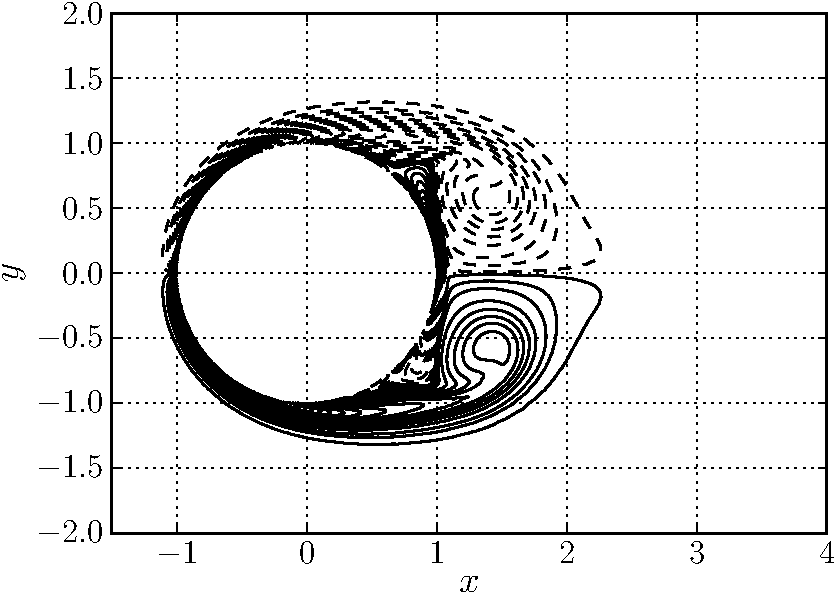
\includegraphics[height=0.2\textheight]{figures/eulerian/ISC_vorticityContours_t3-crop.pdf}
             \caption{$t=3$ Present}
             \label{fig:ISC_vorticityContours_t3-crop}
     \end{subfigure} 
     
     
     \begin{subfigure}[t]{0.45\textwidth}
             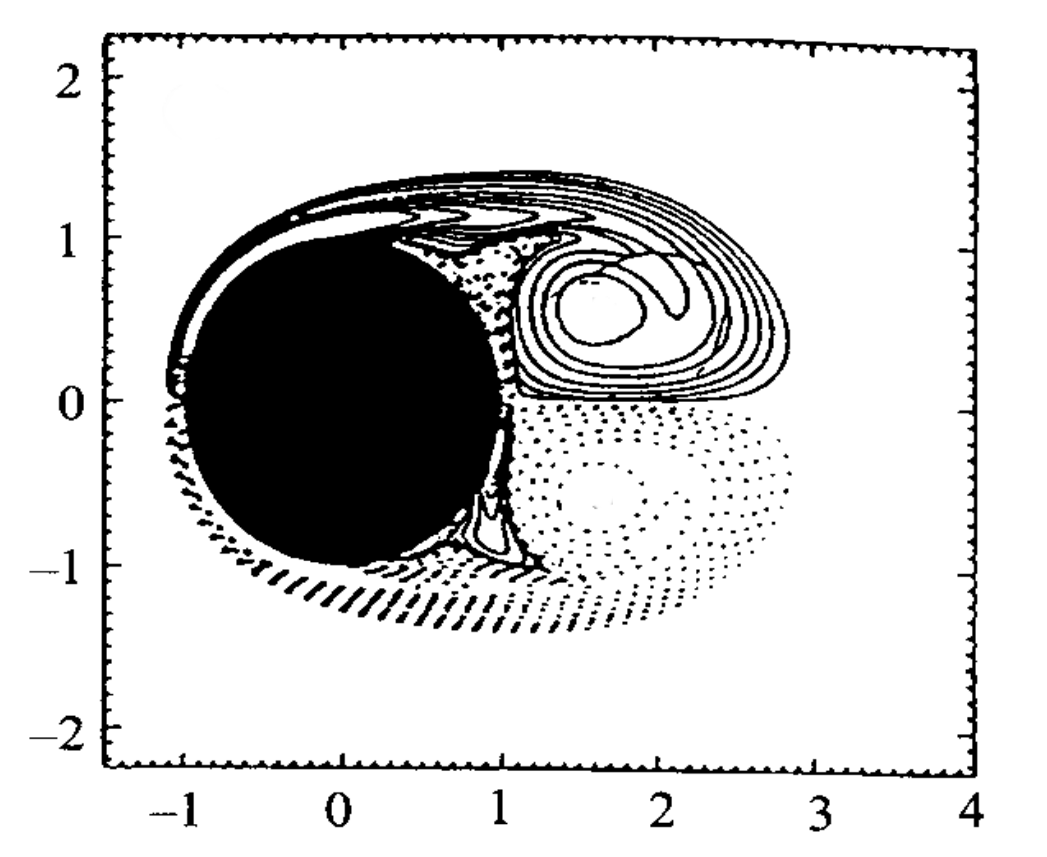
\includegraphics[height=0.2\textheight]{figures/eulerian/ISC_vorticityContours_t5_ref-mod.png}
             \caption{$t=5$ Reference}
             \label{fig:ISC_vorticityContours_t5_ref}
     \end{subfigure}%
     ~ %add desired spacing between images, e. g. ~, \quad, \qquad etc.
       %(or a blank line to force the subfigure onto a new line)
     \begin{subfigure}[t]{0.45\textwidth}
             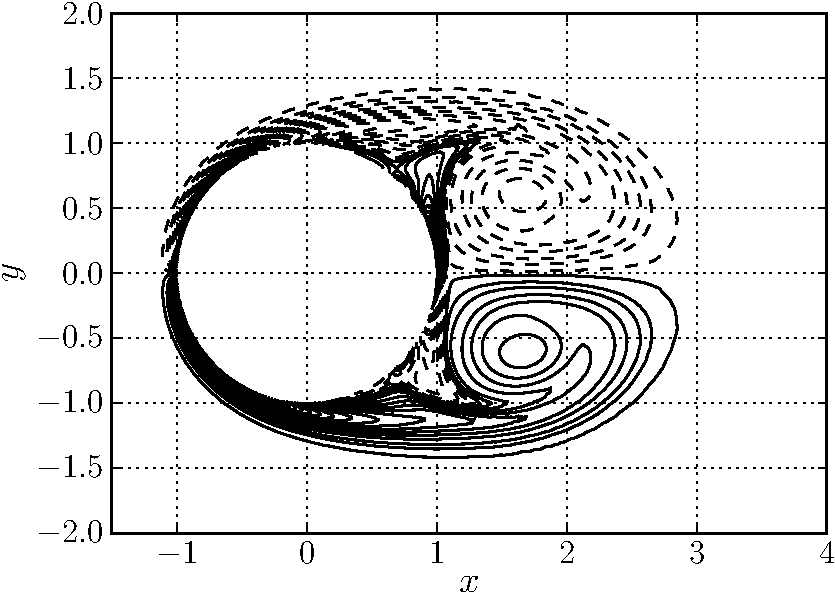
\includegraphics[height=0.2\textheight]{figures/eulerian/ISC_vorticityContours_t5-crop.pdf}
             \caption{$t=5$ Present}
             \label{fig:ISC_vorticityContours_t5-crop}
     \end{subfigure}
     
     \begin{subfigure}[t]{0.45\textwidth}
             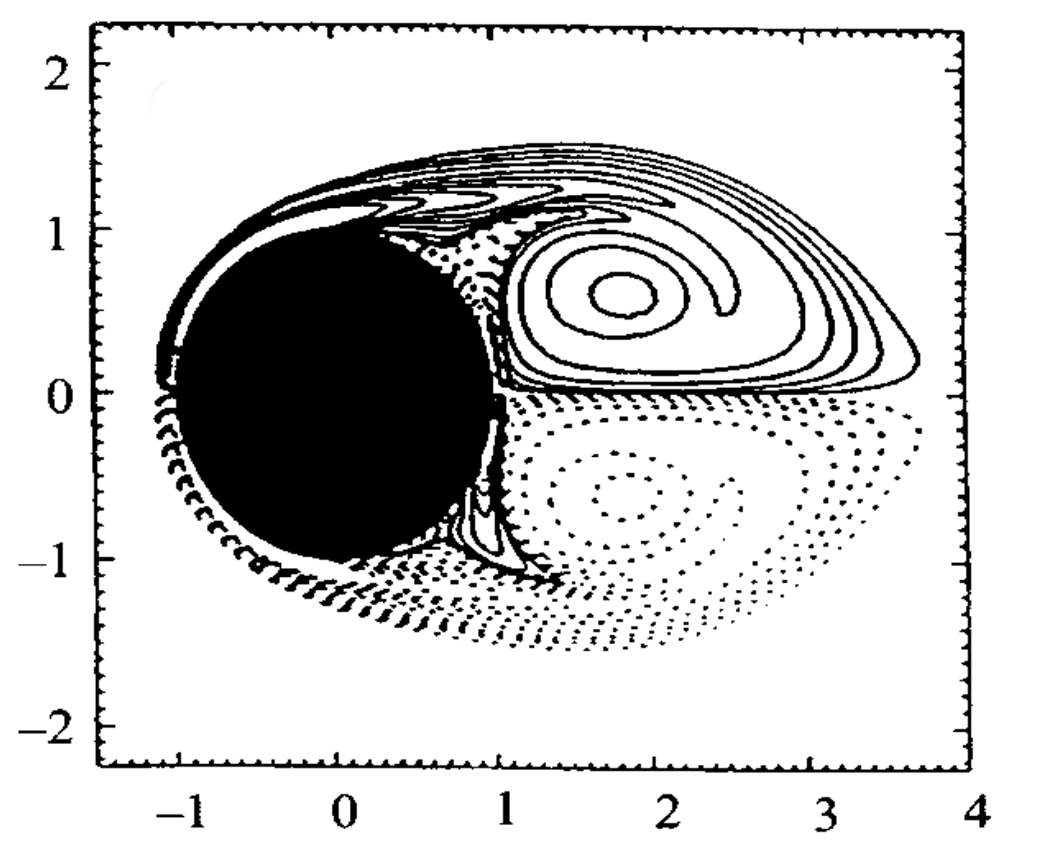
\includegraphics[height=0.2\textheight]{figures/eulerian/ISC_vorticityContours_t7_ref-mod.png}
             \caption{$t=7$ Reference}
             \label{fig:ISC_vorticityContours_t7_ref}
     \end{subfigure}%
     ~ %add desired spacing between images, e. g. ~, \quad, \qquad etc.
       %(or a blank line to force the subfigure onto a new line)
     \begin{subfigure}[t]{0.45\textwidth}
             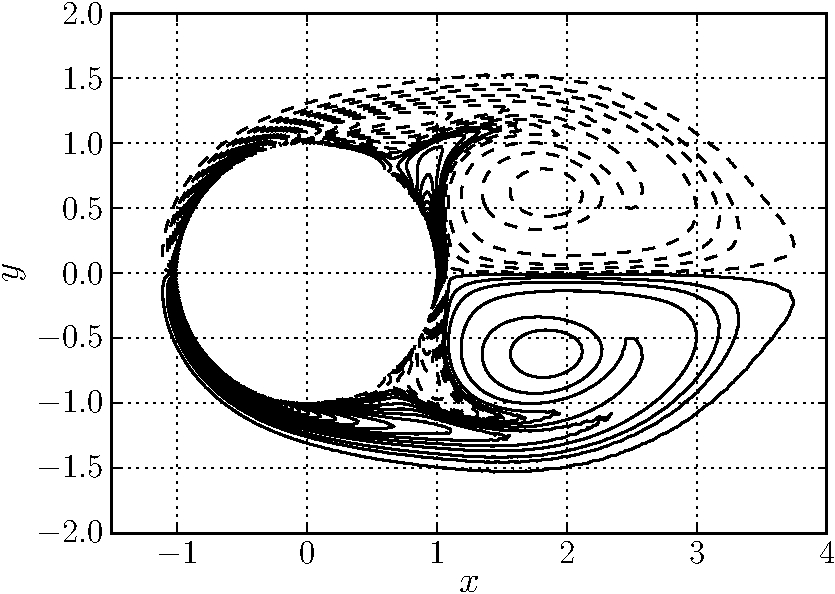
\includegraphics[height=0.2\textheight]{figures/eulerian/ISC_vorticityContours_t7-crop.pdf}
             \caption{$t=7$ Present}
             \label{fig:ISC_vorticityContours_t7-crop}
     \end{subfigure}         

     \caption{Comparison of the vorticity contours for $t=1$, $t=3$, $t=5$ and $t=7$ with contour levels [$-30,...,-2,-1,-0.5,-0.1,0.1,0.5,1,2,...,30$]. The figures on left are obtained from the literature \cite{Koumoutsakos1995a} and the figures on right are from the present study.}
     \label{fig:ISCS_vorticityContours_comparison}
	\end{figure}
	
	\begin{figure}[p]
	\centering
	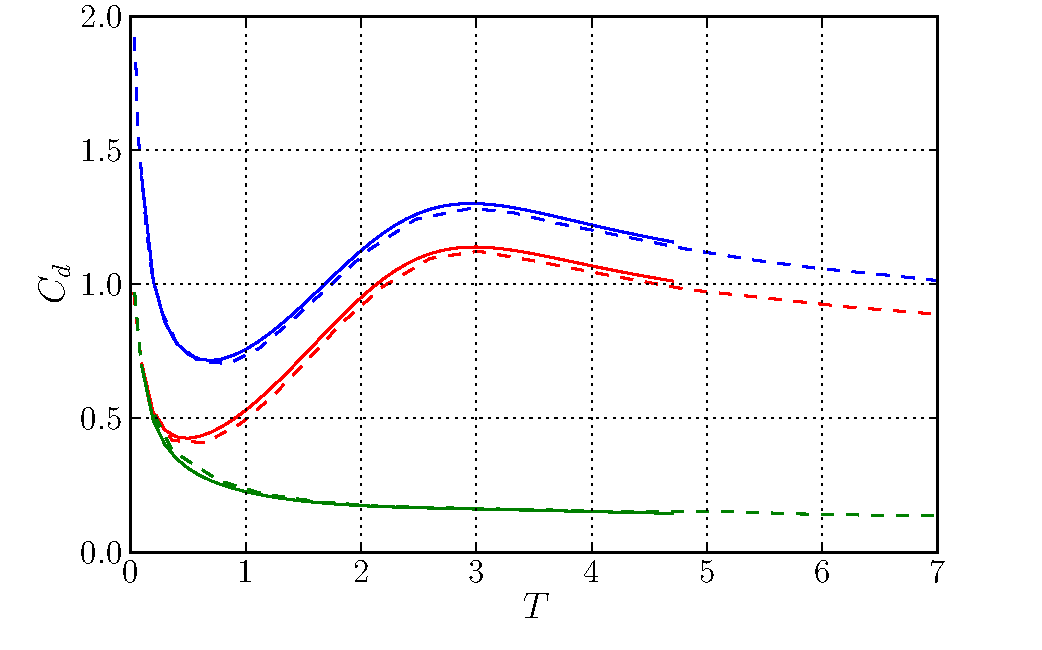
\includegraphics[width=0.7\linewidth]{./figures/eulerian/ISC_dragEvolution.pdf}
	\caption{Evolution of drag force. The figure depicts the total drag coefficient $C_d$ [{\color{plotBlue}{---}}, solid blue], the pressure drag coefficient $C_{d_{\mathrm{pres}}}$ [{\color{plotRed}{---}}, solid red] and the friction drag coefficient $C_{d_{\mathrm{fric}}}$ [{\color{plotGreen}{---}}, solid green]. The dotted lines indicated the data obtained from literature \cite{Koumoutsakos1995a}.}
	\label{fig:ISC_dragEvolution}
	\end{figure}
	
	\begin{figure}[p]
	\centering
	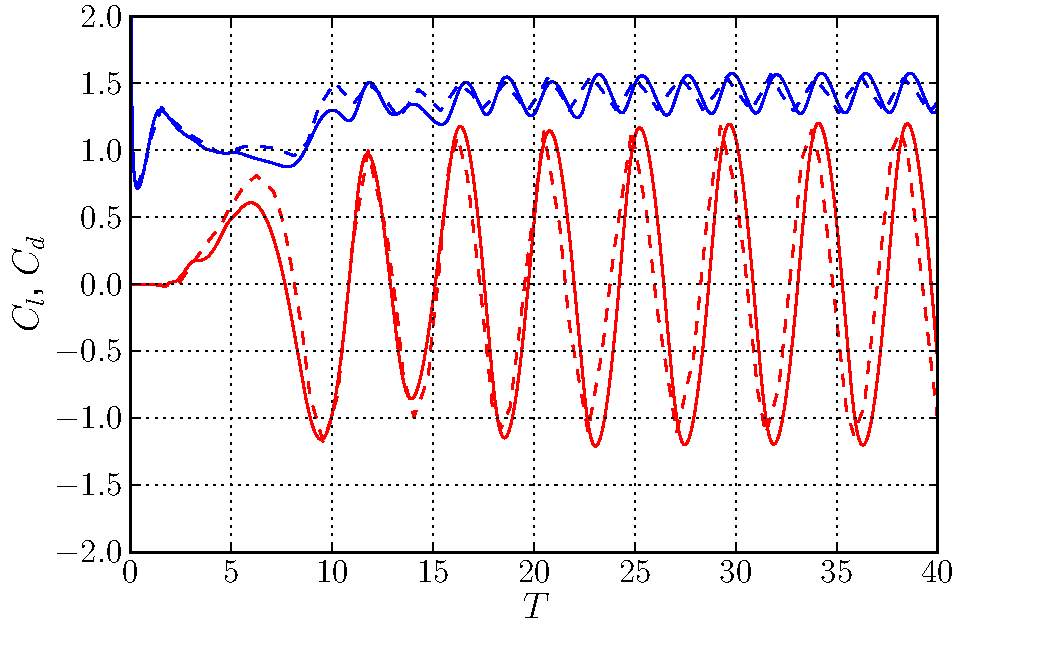
\includegraphics[width=0.7\linewidth]{./figures/eulerian/ISC_LongRun_dragLiftEvolution.pdf}
	\caption{Evolution of the lift and drag coefficient from $t=0$ to $t=40$ with artificial perturbation \cite{Lecointe1984}. The figure depicts the total drag coefficient $C_d$ [{\color{plotBlue}{---}}, solid blue] and the lift coefficient [{\color{plotRed}{---}}, solid red]. The dotted lines represent the data obtained from literature \cite{MosheRosenFeldDochanKwak1991}}
	\label{fig:ISC_LongRun_dragLiftEvolution}
	\end{figure}	

\subsubsection*{Results}
The simulation was started with an with an impulsively started free-stream boundary condition at dirichlet boundary $\partial \Omega_{\mathrm{dirichlet}}$. The problem was evolved from $t=0$ to $t=100$ with number of time steps $N_{\mathrm{tSteps}}=100000$. To validate the scheme with the reference data of Koumoutsakos \& Leonard \cite{Koumoutsakos1995a}, we investigated the evolution of the vorticity field and the evolution of the forces acting on the body.

Figure \ref{fig:ISC_vorticityContours_t7-crop} depicts the evolution of the vorticity from $t=1\rightarrow7$. The iso-vorticity contours of the present study is compared with the reference data from the literature \cite{Koumoutsakos1995a}. At $t=1$, negative and positive vorticity is generated at the top and bottom of the cylinder, respectively and is resulted from satisfying the no-slip boundary condition. As time progress, two primary vortices are formed right behind the cylinder, increasing in shape as time progress. Comparing the vorticity contours, we can say that the shape and the geometry of the contour lines match with the literature. 

Using equations \ref{eq:LiftDragEq} to \ref{eq:LiftDragCoeffEq}, we were able to calculate the Lift and the drag force acting on the cylinder as the time progress, which we used to validate against the literature. Figure \ref{fig:ISC_dragEvolution} shows the components of the drag force (friction drag $C_{d_{\mathrm{fric}}}$, pressure drag $C_{d_{\mathrm{pres}}}$) acting on the surface of the body. At $t=0$, we have a singularity in the total drag $C_d$ acting on the body due to the impulsive start of the flow. It then plunges to $C_d=0.75$ at $t=0.8$ and peaks again near $t=3$ at $C_d=1.3$. The dotted line is the data obtained from literature \cite{Koumoutsakos1995a} and we see that the results of the simulation matches well with the literature.

A final comparison was done for the evolution of the Lift and the Drag coefficient for larger period ($t=0$ to $t=40$), which was used to determine the oscillatory behavior of the Lift and Drag. For lower Reynolds number, the vorticity field is symmetric across the $x$-axis for a long time. This meant that the oscillatory behavior of the forces starts at a much later time. Therefore, we prescribed an artificial perturbation to the problem to create an asymmetry in the vorticity field. The perturbation was performed according to Leocointe \& Piquet \cite{Lecointe1984},
	\begin{equation}
	 u_{\mathrm{wall}} = \begin{cases}
	 0.15 & 3 \leqslant t \leqslant 3.5, \\
	 -0.25 & 3.5 \leqslant t \leqslant 5.
	 \end{cases}
	\label{eq:perturbation}
	\end{equation}
	
With this, we could ensure that we have a controlled behavior for the lift and drag, which we used to determine the amplitude and the frequency of the oscillation. Figure \ref{fig:ISC_LongRun_dragLiftEvolution} compares the evolution of the lift and drag for $t=0$ to $t=40$. We see that our numerical scheme performs very similar to the literature \cite{MosheRosenFeldDochanKwak1991}. However, there is a slight difference, which is due to the under-resolution of the Eulerian domain downstream of the cylinder.

\section{Summary}

In summary, we investigated, verified and validated the Eulerian method for the hybrid coupling scheme, and various observation of the method has been summarized as follows:

	\begin{itemize}
	\item The Eulerian method is used to highly resolve the near-body region of the fluid.
	\item We have used a Finite Element method to solve the incompressible laminar Navier-Stokes problem using the velocity-pressure $\mathbf{u}-p$ formulation.
	\item \printAcron{Incremental Pressure Correction Scheme}{IPCS} was used to solve the Navier-Stokes problem, allowing us to decouple the velocity $\mathbf{u}$ and pressure $p$ from the momentum equation.
	\item \dolfin library from the \fenics project was used to perform automated finite element algorithms for solving the partial different equations.
	\item \gmsh mesh generation tool was used to generate the unstructured mesh of the fluid domain.
	\item Once we have determined the velocity $\mathbf{u}$ and the pressure $p$ fields, we can determine the vorticity associated to the fluid using an optimized calculation algorithm.
	\item A Lamb-Oseen Vortex test case was used to verify the implementation of the Eulerian method, and concluded that the method had a $1^{\mathbf{st}}$-order convergence in time and $2^{\mathrm{nd}}$-order convergence in space.
	\item To validate the vorticity handling and the vorticity production of the no-slip boundary, we used the high-fidelity numerical test case of Clercx \& Bruneau investigation the collision of dipole with the wall at $Re=625$. Investigating the change in kinetic energy $E$, enstrophy $\Omega$, and Palinstrophy $P$, we validate that the results matched the literature. We evaluated the vorticity generated at boundary, which also showed that our numerical method handels according to theory.
	\item The final test case involved simulating an impulsively started cylinder at $Re=550$. We investigated the shed of vorticity at time progress and validated that it matched the reference data provided by Koumoutsakos \& ???. Finally, we investigated the evolution of the Lift and drag of the cylinder, and we saw that the frequency and the amplitude of the oscillation matched the theory. Therefore, our Eulerian method accurate determine the fluid behavior past an object such as the Strouhal number St.
	\end{itemize}

\subsection*{Eulerian method algorithm}

The algorithm for the Eulerian method can be summarized as follows:

	\begin{enumerate}
	\item \textbf{Mesh generation}: We generate the mesh of the fluid domain using \gmsh before the iteration.
	\item \textbf{Determine the boundary condition}: We need to determine the boundary conditions for the boundary domains: $\partial \Omega_{\mathrm{wall}}$, $\partial \Omega_{\mathrm{dirichlet}}$, $\partial \Omega_{\mathrm{pressure}}$. If we have dirichlet velocity boundary conditions for all the exterior boundaries, we do not have to apply any pressure boundary conditions at $\partial \Omega_{\mathrm{pressure}}$.
	\item \textbf{Solve the IPCS}: Using IPCS, time march from $t_n$ to $t_{n+1}$ to solve for the new velocity $\mathbf{u}$ and pressure $p$ field.
	\item \textbf{Determine the vorticity}: Using the algorithm described in \ref{??}, solve for the vorticity field $\omega$ at the time $t_{n+1}$. 
	\end{enumerate}

Once we have the well-resolved vorticity $\omega$ of the near-body region, we use it to couple it with the Lagrangian method with our Hybrid coupling scheme.
